%!TeX program = xelatex

% Define document font, paper size and type %
\documentclass[12pt,a4paper,numbers=noenddot]{scrreprt}

% Include all auxiliary packages
% All required packages to be used within this project

% Margin definitions
\usepackage[a4paper,vmargin=2.5cm,hmargin=3cm]{geometry}

% Packages to be used
\usepackage{fontspec}
\usepackage{eurosym}
\usepackage{amssymb}
\usepackage{mathtools}
\usepackage{upquote}
\usepackage{microtype}
\usepackage{longtable,booktabs}
\usepackage{graphicx}
\usepackage{grffile}
\usepackage{appendix}
\usepackage{float}
\usepackage{pst-all}
\usepackage{geometry}
\usepackage{xcolor}
\usepackage{xpatch}
\usepackage{nccmath}
\usepackage{subcaption}
\usepackage{xcolor}
\captionsetup{compatibility=false}
\usepackage[crop=off]{auto-pst-pdf}
\usepackage[normalem]{ulem}

% Custom links color
\definecolor{linkscolor}{rgb}{0.89, 0.26, 0.2}

\usepackage[unicode=true,bookmarks=true,bookmarksopen=false,
  bookmarksopenlevel=1,pdfborder={0 0 0},backref=false,
  colorlinks=true,allcolors=red,pdfstartview=Fit,
  pdfcenterwindow=true,pdfdisplaydoctitle=true,
  pdfpagelayout=OneColumn,linktocpage=true]{hyperref}
\useunder{\uline}{\ul}{}

% Path for all graphic utilities
\graphicspath{{fig/}}



% Bibliography setup
\usepackage[backend=biber, style=ieee, citestyle=authoryear, sorting=ynt]{biblatex}
\bibliography{bib/articles_modern}
\bibliography{bib/books_classic}
\bibliography{bib/books_modern}

% Custom commands: always the last ones to import to properly override default
% Custom paragraph distance
\setlength{\parskip}{1em plus 2pt minus 1pt}
\setlength{\emergencystretch}{3em}

% Beautiful captions for figures
\captionsetup[figure]{
  format=hang,
  name=Fig.,
  singlelinecheck=off,
  labelsep=colon,
  labelfont=bf,
  font=small
}

% Improve quotations
\newcommand{\quoteauthor}[2]
{
  \begin{flushright}
    \rightskip=1.8cm\textit{``{#1}''} \\
    \vspace{.2em}
    \rightskip=.8cm---{#2}
  \end{flushright}
}

% Improve hyperlinks when citing references
\DeclareCiteCommand{\citetitle}
{\boolfalse{citetracker}%
  \boolfalse{pagetracker}%
  \usebibmacro{prenote}}
{\ifciteindex
  {\indexfield{indextitle}}
  {}%
  \printtext[bibhyperref]{\printfield[citetitle]{labeltitle}}}
{\multicitedelim}
{\usebibmacro{postnote}}

\DeclareCiteCommand{\cite}
{\usebibmacro{prenote}}
{\usebibmacro{citeindex}%
  \printtext[bibhyperref]{\usebibmacro{cite}}}
{\multicitedelim}
{\usebibmacro{postnote}}

\DeclareCiteCommand*{\cite}
{\usebibmacro{prenote}}
{\usebibmacro{citeindex}%
  \printtext[bibhyperref]{\usebibmacro{citeyear}}}
{\multicitedelim}
{\usebibmacro{postnote}}

\DeclareCiteCommand{\parencite}[\mkbibparens]
{\usebibmacro{prenote}}
{\usebibmacro{citeindex}%
  \printtext[bibhyperref]{\usebibmacro{cite}}}
{\multicitedelim}
{\usebibmacro{postnote}}

\DeclareCiteCommand*{\parencite}[\mkbibparens]
{\usebibmacro{prenote}}
{\usebibmacro{citeindex}%
  \printtext[bibhyperref]{\usebibmacro{citeyear}}}
{\multicitedelim}
{\usebibmacro{postnote}}

\DeclareCiteCommand{\footcite}[\mkbibfootnote]
{\usebibmacro{prenote}}
{\usebibmacro{citeindex}%
  \printtext[bibhyperref]{ \usebibmacro{cite}}}
{\multicitedelim}
{\usebibmacro{postnote}}

\DeclareCiteCommand{\footcitetext}[\mkbibfootnotetext]
{\usebibmacro{prenote}}
{\usebibmacro{citeindex}%
  \printtext[bibhyperref]{\usebibmacro{cite}}}
{\multicitedelim}
{\usebibmacro{postnote}}

\DeclareCiteCommand{\textcite}
{\boolfalse{cbx:parens}}
{\usebibmacro{citeindex}%
  \printtext[bibhyperref]{\usebibmacro{textcite}}}
{\ifbool{cbx:parens}
  {\bibcloseparen\global\boolfalse{cbx:parens}}
  {}%
  \multicitedelim}
{\usebibmacro{textcite:postnote}}

\DeclareCiteCommand{\citeauthor}%
{\boolfalse{citetracker}%
  \boolfalse{pagetracker}%
  \usebibmacro{prenote}}
{\ifciteindex
  {\indexnames{labelname}}
  {}%
  \printtext[bibhyperref]{\printnames{labelname}}}
{\multicitedelim}
{\usebibmacro{postnote}}

% Reduce top and lower space in equations
\xpatchcmd{\NCC@ignorepar}{%
  \abovedisplayskip\abovedisplayshortskip}
{%
  \abovedisplayskip\abovedisplayshortskip%
  \belowdisplayskip\belowdisplayshortskip}
{}{}

% Do not restart footnotes counter
\counterwithout{footnote}{chapter}

% Custom norm for equations
\DeclarePairedDelimiter{\norm}{\lVert}{\rVert}


% Start the document
\begin{document}

% Switch off page numbering %
\pagenumbering{Roman}

% Append cover and prologue to actual document %
% Start generating the title page
\begin{titlepage}

  % All content will be centered within this page
  \begin{center}

    % Add cover logo
    \begin{figure}[h]
      \centering
      
\includegraphics[width=\linewidth]{static/banner.png}
    \end{figure}
    \vspace{1cm}

    % Name of the university
    %\textsc{\Large
    %  UNIVERSIDAD CARLOS III DE MADRID
    %}\\[1cm]

    % Nature of the document
    \textsc{\large
      University Degree in Aerospace Engineering
    }\\[0.25cm]
    \textsc{\large
      Academic year 2020-2021
    }\\[1.5cm]
    \textsc{\large
      \textit{Bachelor Thesis}
    }\\[1.75cm]

    % Title of the essay
    \noindent\rule{\textwidth}{1pt}
    \\[0.25cm]
    {
    % Apply font size and color
    \fontsize{35pt}{35pt}\selectfont
    {
      Lambert's problem algorithms: a critical review
    }
    }
    \noindent\rule{\textwidth}{1pt}

    \vspace{1.5cm}
    \textsc{\Large
      Jorge Martínez Garrido
    }\\[4cm]
    \textsc{\large
      Supervised by:
    }\\[0.25cm]
    \textsc{\large
      Manuel Sanjurjo Rivo
    }\\[3cm]

    % Author of the essay
    %\begin{table}[ht]
    %  \centering
    %  \begin{tabular}{cc}
    %    {\ul \Large \textbf{Author}}   & {\ul \Large \textbf{Supervisor}} \\
    %    \multicolumn{1}{l}{}           & \multicolumn{1}{l}{}             \\
    %    \large{Jorge Martínez Garrido} & \large{Manuel Sanjurjo Rivo}
    %  \end{tabular}
    %\end{table}

    \textsc{\large
       September, 2021
    }\\[0.25cm]
    \textsc{\large
       Leganés (Madrid)
    }\\[0.25cm]

  \end{center}
\end{titlepage}

\chapter*{Abstract}

This work presents a deep performance comparison from both the analytical and
computational point of view of a variety of modern Lambert's problem solvers.
The analyzed solvers are \cite{gauss1809}, \cite{battin1984},
\cite{gooding1990}, \cite{avanzini2008}, \cite{arora2013}, \cite{vallado2013}
and \cite{izzo2015}.

A quick review on the problem's timeline, geometry, possible solutions and
singularities are presented at first. This is followed by an explanation on the
different elements required by any solver together with a proposed way on how to
classify these algorithms.

Each selected solver is analyzed considering the free-parameter employed, the
initial guess procedure, the numerical root solver and the way velocity vectors
are constructed. Figures for the time of flight as function of the independent
variable are provided.

The performance comparison is carried out for all possible combinations of the
transfer angle and non-dimensional time considering the total number of
iterations, the time per iteration and the total computation time. The results
are provided in the form of contour plots. A resume table with a conclusion on
the obtained results is included too.

Finally, some ideas about how the performance comparison could be extended and
enhanced are included in the last chapter.

\vspace{4cm}
\textbf{Keywords:} Lambert's problem, two-body problem, orbital boundary value
problem, algorithms.


% Start the table of contents %
\tableofcontents

% ---------- BEGIN OF CONTENT FILES -------------

% --------------------------------- %
% --- INTRODUCTION TO THIS WORK --- %
% --------------------------------- %
\chapter{Introduction to this work}
\pagenumbering{arabic}

This first chapter is devoted to some introductory concepts about the problem
being addressed, the different procedures used and the goals achieved. All these
items will help the reader to have a better understanding of the project's
structure. In addition, a collection of real-world applications together with a
brief socioeconomic analysis are presented in the last sections in order to
justify the importance of the problem in today's world.

% --- Sections for this chapter --- %
% --- PROBLEM DESCRIPTION --- %
\section{Problem description and motivation}

The two-body boundary value problem in the framework of orbital mechanics and
astrodynamics is known as the Lambert's problem. Solutions to this problem find
the orbit which connects two known positions vectors over a finite time of
flight.

\begin{figure}[H]
  \centering
  \includegraphics[scale=1]{problem_geometry.png}
  \caption{
    The geometry of the Lambert's problem as seen from an inertial frame
    centered in the orbit's attractor. Observation vectors are labeled as
    $\vec{r_{1}}$ and $\vec{r_{2}}$, being $\Delta \theta$ the angle between
    them and $\Delta t$ the epoch difference.
  }
  \label{fig:problem_geometry}
\end{figure}

Since its formulation almost 300 years ago, a plethora of solutions have been
proposed. Nevertheless, the problem is still of interest due to its applications
(see section \ref{sec:applications}) and many modern authors have addressed it
by developing new numerical techniques. Therefore, when it comes to solve for
the Lambert's problem, a big set of algorithms is available and the following
question arises: which one of those performs the best under particular given
conditions. The search for a solution to previous question is the motivation
behind this work.

% --- OBJECTIVES AND GOALS --- %
\section{Objectives and goals achieved}

The main objective of this project is a critical review and comparison on the
most popular solvers for the Lambert's problem. To achieve this purpose, the
whole process was divided into the following key objectives:

\begin{itemize}

  \item \textbf{Review of Lambert's problem timeline.}
        The historical background showed which authors have proposed solutions
        to the problem and when they did so. Important scientific
        figures arose when carrying out this part of the research.

  \item \textbf{Analysis of problem's geometry, solutions and singularities.}
        A deep review on the problem was performed by listing all the
        different solutions their nature.  Multi-revolution transfers were also
        considered together with limiting cases.

  \item \textbf{Collection of modern algorithms.}
        A mathematical comparison between all of them was carried out taking
        into account four factors: the selected iteration variable, the
        numerical method used, proposed initial guess and the way of
        computing the velocity vectors.

  \item \textbf{Implementation of a new method.}
        A new routine based on the analytical solution to the conic equations
        was implemented for the first time and compared against previous
        solvers too.

  \item \textbf{Performance framework and comparison.}
        All computer algorithms were coded under the same programming language,
        so no undesired additional performance was introduced.  Contour
        maps relating the transfer angle, time of flight and number of
        iterations to achieve desired accuracy were computed to
        illustrate the robustness of each routine.

  \item \textbf{Discussion on the obtained results.}
        Strengths and weaknesses of each algorithm were exposed with previous
        analysis. All the results were collected and studied to raise
        new ideas regarding solutions performance of future solvers.

\end{itemize}

The implementation of all collected algorithms lead to the creation of a
Lambert's problem solvers hub in the form of a software
library\footnote{Available under public license at:
  https://github.com/jorgepiloto/lamberthub}, which will be useful for other
authors when testing new numerical procedures.

% --- REAL-WORLD APPLICATIONS --- %
\newpage
\section{Real-world applications}
\label{sec:applications}

Lambert's problem solvers have lots of applications because they retrieve the
solution to the \textit{boundary value problem} (BVP) of the restricted two-body
dynamics problem.  This solution is nothing but the conic trajectory which the
body will follow as time evolves. The previous fact makes Lambert's problem to be
usually included within the initial \textit{orbit determination topic} (IOD).

However, the most common applications for the Lambert's problem are targeting,
maneuvering and rendezvous ones. For example, if it is desired to navigate from
an initial position to a final one over a finite amount of time then, the orbit
which must be followed is the one obtained by solving the Lambert's problem.

In fact, Lambert's solvers routines were implemented in the \textit{Apollo
  Guidance Computer} (AGC\footnote{The original source code for the AGC has been
  published under a Public Domain license in
  https://github.com/chrislgarry/Apollo-11}) for the calculation of transfer
trajectories and reentry ones. In the \citetitle{apollo1972}, it is claimed that
the algorithms (AGC programs P-31 to P-37) took between 15 to 30 minutes to
compute a solution, which showed the necessity of having better performance
solvers for future missions.

% Example of Apollo Lunar Module rendezvous %
\vspace{0.5cm}
\begin{figure}[h]
  \centering
  \includegraphics[scale=1]{apollo_trajectory.png}
  \caption{After the \textit{Lunar Module} (LM) was launched into a
    \textit{Constant Delta Height} (CDH) orbit, a set of targetting
    maneuvers were required to perform a rendezvous with the \textit{Command
      and Service Module} (CSM). The AGC made use of its own Lambert's
    solvers routines to calculate the required impulses in order to correct
    the course of the LM spacecraft.}
  \label{fig:apollo_trajectory}
\end{figure}

Course corrections, as shown in figure \ref{fig:apollo_trajectory}, might be
required during the transfer, forcing to compute a new solutions by calling the
different transfer routines several times in order to reach final aiming
location.

Last application is closely related with the mission analysis field. Solving
Lambert's problem for a given set of launching and arrival dates leads to a
collection of particular orbits, each one corresponding to a transfer arc.
Those conic trajectories show a different characteristic velocity, directly
related with the amount of required energy.  Contour maps representing this set
of solutions are known as porkchop plots and it is possible to observe that minimum
transfer points exist within these figures.  These locations in the contour
figure are usually selected for space missions launch and arrival dates.

% Figure showing optimal transfer for Mars perseverance
\begin{figure}[h]
  \centering
  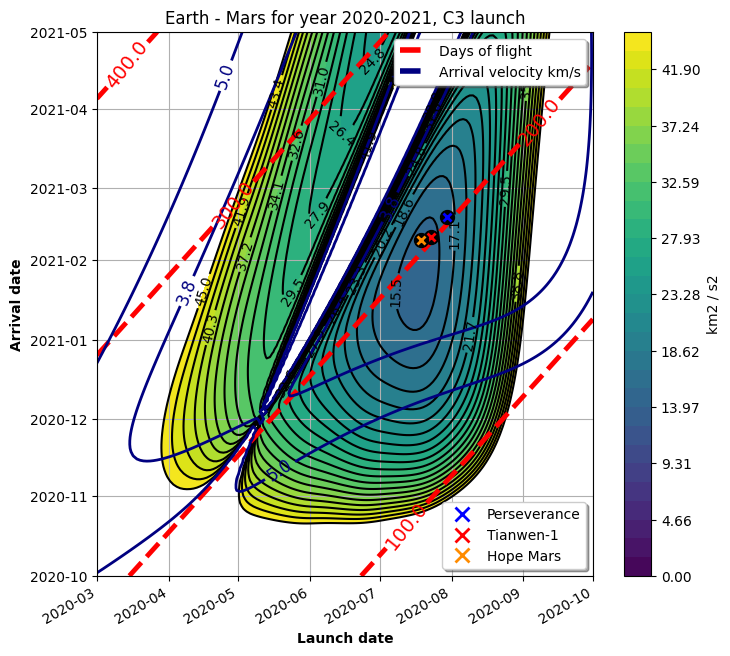
\includegraphics[width=\linewidth]{static/porkchop.png}
  \caption{Porkchop for Earth-Mars transfer arrival energy for years 2020-2021.
    Each point in the figure is obtained by solving the Lambert's problem in order
    to compute departure $C_{3}$ (characteristic energy). Notice the optimal
    transfer dates are being used by latest missions about this planet:
    \cite{perseverance2020}, \cite{tianwen1} and \cite{hope2021}.}
  \label{fig:porkchop_perseverance}
\end{figure}

With all previous examples on mind, it is clear that Lambert's applications
require from high performance solving routines to compute in a fast and reliable
way final desired orbit trajectories.

% --- SOCIAL AND ECONOMICAL CONTEXT --- %
\section{Social and economical context}

During the last decades, the amount of unmanned spacecrafts orbiting our planet
has dramatically increased. The main reason behind this situation is the rise of
private launchers and manufacturers, who have lowered the costs, enabling others
to get access to space. This lead to a new aerospace race driven by cheap
technologies, usually referred to as \textit{New Space}, which provide agile,
responsive and cheaper solutions to common aerospace tasks.

In addition, a huge demand of communication services is already being experience
by the aerospace market.  Nowadays, this sector generates benefits over $100$
billion euros due to new improvements in satellites' software and hardware.
Communication services have a variety of purposes, from in-flight connectivity
to network-centric warfare, which are fulfilled by making use of satellite
constellations in order to guarantee a permanent coverage over particular areas
of the globe.

% Reference
% https://www.airbus.com/public-affairs/brussels/our-topics/space/new-space.html

\begin{figure}[h]
  \centering
  \includegraphics[width=\linewidth]{sat_evolution.png}
  \caption[Launched satellites per year.]{Amount of satellites launched during last decades and filtered by their
    mission purpose: space science, Earth observation and communication. This
    last one, shows a big growth rate specially during the last five years. Data
    was obtained and processed from the UCS Satellite Database.}
  \label{fig:sat_evolution}
\end{figure}

All previous satellites' missions, shown in figure \ref{fig:sat_evolution}, are
designed to take place at particular locations of space, as some of those orbits
require specific altitudes and inclinations: geostationary, sun-synchronous...
However, space is a very hostile environment and orbit perturbations exist due
to air drag, Earth's oblateness, third body presence or solar radiation pressure
among many others. These perturbations might originate a shift in the initial
orbit, making it necessary to maneuver the satellite to original desired
position. Orbit corrections require from targeting algorithms which, in the end,
are Lambert's problem solvers.

Within the frame of aerospace sector, a new professional profile is being
demanded by companies: the computer scientist. These people are usually
engineers who have a deep knowledge in both high-performance computing and
mathemtatics modelling the problem. This is one of the reasons behind why many
modern papers, which devise a new approach for the Lambert's problem, include
algorithms in the form of code flowcharts, pseudo-code or links to repositories
hosting original source computer routines.

\begin{figure}[h]
  \centering
  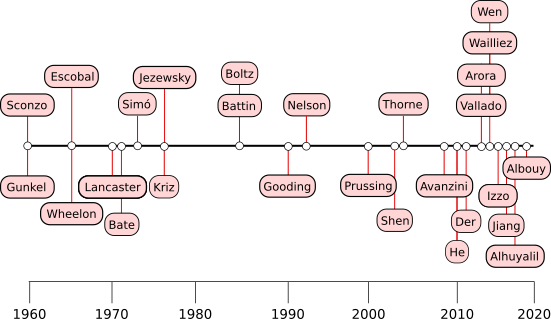
\includegraphics[width=\linewidth]{static/solvers_timeline.png}
  \caption[Publications related with Lamebert's problem.]{More than a dozen of papers have been published over the last twenty
    years. The nature of the proof solutions has evolved also during time, going
    from pure geometric demonstrations to graphic processing units based or even machine
    learning ones.}
  \label{fig:art_lambert}
\end{figure}



% --------------------------------- %
% ---      PROBLEM REVIEW       --- %
% --------------------------------- %
\chapter{Review of Lambert's problem}
\label{sec:review_lambert}

In this chapter, the problem statement, geometry, solutions and singularities
are revisited. The analysis presented here is strongly influenced by
\cite{escobal1965}, \cite{el1968} and \cite{battin1999} works. All scenarios,
including multiple revolutions and degenerate ones are considered.

% --- Sections of this chapter --- %
\section{The statement of the problem}

Lambert's problem states to find for the Keplerian orbit which connects two
known position vectors, $\vec{r_{1}}$ and $\vec{r_{2}}$, over a finite amount of
time, $\Delta t$, under a gravity field of intensity $\mu$. The
three-dimensional representation of this problem was initially introduced by
figure \ref{fig:problem_geometry}. This problem is usually named \textit{the
  direct-arc transfer problem}.

Previous statement is the most common one when addressing the problem. However,
it is also possible to specify the number of revolutions of the orbiting body
before reaching the final position vector. This type of problem is known as
\textit{the multi-revolution problem}.

It is important to say that perturbations will not be considered during this
whole work: only the Keplerian Lambert's problem is studied.

Because the answer to either the direct-arc transfer of the multi-revolution one
is an orbit, we then need a total of six parameters (3 translations + 3
rotations) to fully describe its shape, location and orientation. These set of
parameters is usually referred to as \textit{orbital elements}. Two of the most
common ones are:

\begin{itemize}
  \item RV set: composed by the three components of the initial position
        vector $\vec{r_{1}}$ and the other three components of the
        initial velocity vector $\vec{v_{1}}$.
  \item COE set: known as the \textit{classic orbit elements}. The
        elements which form this set are the semi-major axis $a$, the
        orbit's eccentricity $e$, its inclination $i$, right ascension
        of the ascending node $\Omega$, argument of the perigee $w$ and
        finally the true anomaly denoted by $\nu$.
\end{itemize}

Therefore, the Lambert's problem is solved once a full set of orbital elements
is retrieved, as the orbit between the two known position vectors is finally
known.

\section{The orbital plane}

Assuming that the time of flight is not null, and that the position vectors are
not coincident neither forming an angle of $180$ degrees between them, the whole
orbit movement will be contained within a plane. This plane is usually named the
orbital plane. The red colored plane in figure
\ref{fig:problem_geometry} represents it.

For the case of the Lambert's problem, the orbital plane can be computed
from the initial and final position vectors. These two vectors form a basis from
which any other vector contained in the plane can be obtained from the relation
shown in equation \ref{eq:linear_combination}:

\begin{equation}
  \vec{r} = a \vec{r_{1}} + b \vec{r_{2}}
  \label{eq:linear_combination}
\end{equation}

where $a$ and $b$ are two known real values.

As long as both vectors are linearly independent, the orbital plane is defined.
This implies that the cross product $\vec{r_{1}} \times \vec{r_{2}}$ must be not
null, otherwise singularities arise. This justifies previous assumption about
not having two position vectors which might be parallel (i.e. forming $0$ or
$180$ degrees).

The orientation of the orbital plane in space with respect to (w.r.t.) is
given by the right ascension of the ascending node (RAAN) $\Omega$ and the
inclination $i$ elements. Therefore, it is interesting to analyze the Lambert's
problem by making use of the COE set instead of the RV one.

Because both the RAAN and the inclination are computed from a vector in the
direction and sense of the specific angular momentum of the orbit, $\vec{h}$,
the following subsection presents a simple procedure on how to solve for this
particular vector.


\subsection{Solving for the unitary specific angular momentum vector}

It is not possible to compute the specific angular momentum of the orbit because
a velocity at a particular point would be required. This condition would satisfy
the RV set, meaning that the orbit is fully determined. However, a unitary
vector in the direction and sense of the angular momentum can be computed making
use of the two knwon position vectors and the sense of motion of the observed
body.

The sense of motion (prograde or retrograde)\footnote{Prograde and retrograde
  orbits are defined according if their inclinations are lower or greater than
  $90$ degrees respectively.} is an important parameter, since it fixes the sense
of the angular momentum of the orbit. The reason is that, when computing a
normal vector to the normal plane via equation \ref{eq:normal_vector}

\begin{equation}
  \vec{h_{0}} = \frac{\vec{r_{1}} \times \vec{r_{2}}}{\norm{\vec{r_{1}}}\norm{\vec{r_{2}}}}
  \label{eq:normal_vector}
\end{equation}

the resultant normal vector has always the sense imposed by the so-called
\textit{right hand rule} according to the shortest angle between $\vec{r_{1}}$
and $\vec{r_{2}}$. In addition, notice that vector $\vec{h_{0}}$ goes in the
direction of the $\vec{h}$ vector, but does not have neither its sense or
magnitude.

Therefore, the value of $\vec{h_{0}}$ needs to be corrected according if it does
not agree with a prograde/retrograde type of motion observed. This implies
checking for the sign of the third component of via $h_{0_{Z}} =
  \vec{k} \cdot \vec{h_{0}}$ and apply:

\vspace{0.15cm}
\bgroup
\def\arraystretch{1.5}
\begin{table}[H]
  \centering
  \begin{tabular}{|c|c|c|}
    \hline
    \textbf{Sign of the vertical component} & \textbf{Prograde} & \textbf{Retrograde} \\ \hline
    $h_{0_{Z}} > 0$                         & $\vec{h_{0}}$     & $-\vec{h_{0}}$      \\ \hline
    $h_{0_{Z}} < 0$                         & $-\vec{h_{0}}$    & $\vec{h_{0}}$       \\ \hline
  \end{tabular}
  \caption{Sign correction for the normal specific angular momentum vector.}
\end{table}
\egroup

where vector $\vec{k}$ in the dot product operation is a unitary one in the
direction and sense of the positive $Z$ axis of the inertial reference frame
selected to study the problem.

With previous correction, the resultant vector $\vec{h_{0}}$ goes in the
direction and sense of the specific angular momentum one but has unitary
modulus.

\subsection{Solving for the inclination of the orbit}

Once $\vec{h_{0}}$ has been computed and its sign properly fixed, the
inclination of the orbit can be computed by making use of expression
\ref{eq:inclination_orbit}:

\begin{equation}
  i = \arccos{\left(\frac{h_{0_{Z}}}{\norm{\vec{h_{0}}}} \right)}
  \label{eq:inclination_orbit}
\end{equation}

Because the sign correction was previously applied, the value of the inclination
must agree with the prograde/retrograde type of motion. Furthermore, the output
of the $\arccos$ function is bounded to the inclination domain (i.e. $0$ and
$\pi$ radians).


\subsection{Solving for the RAAN of the orbit}

Finally, the right ascension of the ascending node is computed as usual. First,
a vector in the direction of the line of nodes is computed taking advantage of
the expression \ref{eq:line_of_nodes}:

\begin{equation}
  \vec{n} = \vec{k} \times \vec{h_{0}}
  \label{eq:line_of_nodes}
\end{equation}

With previous vector, it is possible now to compute the RAAN by applying
equation \ref{eq:raan}

\begin{equation}
  \Omega = \arccos{\left(\frac{\vec{i} \cdot \vec{n}}{\norm{\vec{i}}
      \norm{\vec{n}}}\right)}
  \label{eq:raan}
\end{equation}

where vector $\vec{i}$ in the dot product operation is a unitary one in the
direction and sense of the positive $X$ axis of the inertial reference frame
selected to study the problem.

Because the RAAN is bounded between $[0,2\pi)$, a correction might be required,
as the $\arccos$ function only returns values between $[0,\pi)$. This correction
is triggered if the lateral component of the line of nodes, $\vec{n_{j}} < 0$,
so the final value of $\Omega$ becomes:

\begin{equation}
  \Omega = 2\pi - \Omega \Rightarrow \vec{n_{j}} < 0
  \label{eq:raan_correction}
\end{equation}

From the point of view of a computer routine, it is better to make use of the
$\arctantwo$\footnote{This routine was originally introduced by the FORTRAN
  language under the name of $\atantwo$.}, which returns the proper quadrant
between the input coordinates, so the RAAN can be easily computed following
relation \ref{eq:raan_computer}:

\begin{equation}
  \Omega = \arctantwo(n_{y}, n_{x})
  \label{eq:raan_computer}
\end{equation}

where $n_{y}$ and $n_{x}$ are the lateral and longitudinal coordinates of the
line of nodes vector.

Once $\Omega$ has been solved together with $i$, the complete orientation in
space of the orbital plane is known.

\subsection{The problem as seen from the orbital plane}

Because the orbital plane is completely known, only the following parameters are
still required to solve for the orbit: $a$, $e$, $w$ and $\nu$. Notice that the
true anomaly, that is $\nu$, only gives information about the current location
of the body along its orbit but not about the shape of the orbit itself.
Therefore, the problem is just devoted to find the values of $a$, $e$ and $w$.

Since all the motion of the problem is contained in the orbital plane, it is
feasible to study the Lambert's problem a reference who's $z=0$ plane is
coincident with previous plane. Reader might have thought about using the
\textit{perifocal coordinate system} (PQW) but the argument of perigee is still
an unknown of the problem, so it is not possible to use the PQW frame. With
previous assumption, we can simplify the geometry given by figure
\ref{fig:problem_geometry} into the one shown by figure
\ref{fig:lambert_problem_pqw}.

\vspace{0.15cm}
\begin{figure}[H]
  \centering
  \includegraphics[scale=1]{lambert_problem_pqw.png}
  \caption{
    The geometry of the Lambert's problem as seen from an inertial frame who's
    $XY$ plane coincides with the orbital one..
  }
  \label{fig:lambert_problem_pqw}
\end{figure}

Notice that the attracting body in figure \ref{fig:lambert_problem_pqw} is
located in the known focus $F$, following the two-body dynamics assumption. The
other focus $F'$ is still unknown and needs to be solved to retrieve the full
geometry of the orbit. This also introduces the unknown of the $w$, as the line
where for the semi-major needs to be guessed.



\section{Lambert's theorem and implicit solution}
\label{sec:lamberts_theorem}

The Lambert's problem receives its name after Johann Heinrich Lambert formulated
it in a letter to Leonhard Euler, see APPENDIX XX for more information about
Lambert's problem origin and timeline.

Lambert proof in his \citetitle{lambert1761} that the time of flight between two
position vectors only depends on the sum of these radial distances, the linear
distance between them and the semi-major axis of the orbit. This is known as
\textit{the Lambert's theorem}.

\subsection{The vis-viva equation in its differential form}

To demonstrate Lambert's theorem, the original procedure devised by him is
presented in the following lines. Starting from the vis-viva equation in
\ref{eq:visviva}:

\begin{equation}
  v = \frac{dr}{dt} \sqrt{\frac{2\mu}{r} - \frac{\mu}{a}}
  \label{eq:visviva}
\end{equation}

it is possible to integrate to find that:

\begin{equation}
  \Delta t = \frac{1}{\sqrt{\mu}} \int_{s-c}^{s} \frac{r dr}{\sqrt{2r -
      r^{2}/a}}
  \label{eq:visviva_integral}
\end{equation}

where in previous equation $s$ is the semi-perimeter and $c$ the chord, being
given by:

\begin{equation}
  s = \frac{\norm{\vec{r_{1}}} + \norm{\vec{r_{2}}} +
    \norm{\vec{c}}}{2}\quad\quad\quad\quad
  \vec{c} = \vec{r_{2}} - \vec{r_{1}}
  \label{eq:s_and_c_lambert}
\end{equation}

\subsection{Series solution to the vis-viva differential equation}

Lambert provided equation \ref{eq:visviva_integral} in the form of a
series\footnote{This equation has been directly taken from \cite{battin1999}, in
  particular from problem 7-1 of the book.}: \ref{eq:visviva_series}:

\begin{flalign*}
  \Delta t = \frac{1}{\sqrt{\mu}} \left(\frac{\sqrt{2}}{3}[s^{\frac{3}{2}}\mp (s-c)^{\frac{3}{2}}] \right. &  &
\end{flalign*}

\vspace{-1.25cm}
\begin{equation}
  \left. +\sum_{n=1}^{\infty}\frac{\sqrt{2}}{2n+3}\frac{(2n-1)!}{2^{3n-1}n!(n-1)!}[s^{n+\frac{3}{2}} \mp (s-c)^{n+\frac{3}{2}}]\frac{1}{a^{n}}\right)
  \label{eq:visviva_series}
\end{equation}

However, notice that for solving the value of the semi-major axis a numerical
method is required, as equation \ref{eq:visviva_series} is not in explicit form
for $a$.

Lambert told Euler that he would devise the explicit form of
\ref{eq:visviva_series} (see \cite{albouy2019}) but Lambert's untimely death
prevented this.

\section{Geometry of the solutions}

Before introducing or proposing any mathematical method for solving equation
\ref{eq:visviva_series}, we will assume that we managed somehow to obtain the
right value for the semi-major axis of the orbit.

With this value, it is possible to identify the type of orbit, according to the
following table:

\begin{table}[H]
  \centering
  \begin{tabular}{|c|c|c|}
    \hline
    \textbf{$0 < a < \infty$} & \textbf{$a = \infty$} & \textbf{$a < -\infty$} \\ \hline
    Elliptic                  & Parabolic             & Hyperbolic             \\ \hline
  \end{tabular}
  \caption{Type of orbit according to semi-major axis value.}
\end{table}

Knowing the value of $a$ it is possible to estimate the rest of the orbital
elements so the observed orbit is fully determined. However, each type of orbit
requires from its own solution procedure when determining the eccentricity,
argument of perigee and the current true anomaly.

Therefore, in the following subsections, the possible solutions and procedures
for each type of orbit are exposed from a geometrical point of view.

\subsection{The elliptic transfer geometry}

An elliptic orbit has a semi-major axis who's value lies between $[0,\infty)$
units of length. By recalling that:

\begin{equation}
  \overline{FP} + \overline{F'P} = 2a
  \label{eq:ellipse_property}
\end{equation}

being $\overline{FP}$ and $\overline{F'P}$ the distance to the
primary\footnote{The primary focus is the one in which the attractor is placed.}
and vacant\footnote{Named like this because it does not hold the attractor.}
focus, it is possible to find the location of this last one.

In order to achieve previous task, we make use of equation
\ref{eq:ellipse_property} and evaluate it for each known position vectors:

\begin{equation}
  r'_{1} = 2a - r_{1}\quad\quad
  r'_{2} = 2a - r_{2}
\end{equation}

The values $r'_{1}$ and $r'_{2}$ indicate the distance at which the vacant focus
$F'$ is located. Therefore, by tracing a circumference of radius $R_{1} = r'_{1}$
centered at the tip of vector $\vec{r_{1}}$ and another with $R_{2} = r'_{2}$ at
the tip of vector $\vec{r_{2}}$ it is possible to find graphically where the
vacant focus is located.

\subsubsection{Two vacant focus}
When both circumferences cross at two points, meaning there are two possible
vacant focus, as shown by figure \ref{fig:elliptic_geometry_1}. Having two focus
means having two elliptic paths and a total of four orbits:

\begin{itemize}
  \item Red orbit and prograde motion.
  \item Red orbit and retrograde motion.
  \item Blue orbit and prograde motion.
  \item Blue orbit and retrograde motion.
\end{itemize}

By imposing the sense of motion to be prograde or retrograde, the solution space
is reduced to two possible orbits. To distinguish between the two, we introduce
a new parameter named \textit{the orbit path}, which enables us to select
between one or the other. See section XX for more information about the orbit
path.

In this scenario, it holds that:

\begin{equation}
  a > \frac{\norm{\vec{r_{1}}} + \norm{\vec{r_{2}}} + \norm{\vec{c}}}{4}
\end{equation}

Finally, it must be said that these solution only appear in the
multi-revolution problem.

\begin{figure}[H]
  \centering
  \includegraphics[scale=1]{geometry_elliptic1.png}
  \caption{
    In this scenario, there are a total of four solutions considering two
    possible orbits (blue and red) and the transfer angle (lower or greater than
    180 degrees), which is equivalent to prograde or retrograde motion. Fixing
    the type of motion together with the orbit path parameter will retrieve the
    current solution to the problem.
  }
  \label{fig:elliptic_geometry_1}
\end{figure}

\subsubsection{One vacant focus}
In this case, both circumferences are tangent to each other, meaning there is
only one common point and thus a single vacant focus. See figure
\ref{fig:elliptic_geometry_2} for a graphical representation.

In this case, only two solutions can be achieved:

\begin{itemize}
  \item Red orbit and prograde motion.
  \item Red orbit and retrograde motion.
\end{itemize}

Similarly to previous case, imposing the sense of motion will retrieve the
current solution to the problem. Notice now that the orbit path parameter is no
longer required as only one orbit (red one) exists.


For this scenario, the semi-major axis is found to be:
\begin{equation}
  a = \frac{\norm{\vec{r_{1}}} + \norm{\vec{r_{2}}} + \norm{\vec{c}}}{4}
\end{equation}

A single vacant focus is likely to appear for the direct arc transfer problem.

\begin{figure}[H]
  \centering
  \includegraphics[scale=1]{geometry_elliptic2.png}
  \caption{
    In this scenario, there are only two solutions considering a single orbit
    (red one) and the transfer angle (lower or greater than 180 degrees),
    equivalent to prograde or retrograde motion. Fixing the type of motion will retrieve the current solution to the problem.
  }
  \label{fig:elliptic_geometry_2}
\end{figure}


\subsubsection{No vacant focus}
In this last situation, there is not a common point between the two
circumferences, meaning that the transfer orbit does not exist for that
particular geometry.

In fact, the semi-major axis turns out to be:
\begin{equation}
  a < \frac{\norm{\vec{r_{1}}} + \norm{\vec{r_{2}}} + \norm{\vec{c}}}{4}
\end{equation}

meaning that the problem is unsolvable.

\subsubsection{Computing the rest of the elements in the elliptic case}
Once the location of the vacant focus has been identified, it is possible to
solve for the focal distance $c$ by applying equation \ref{eq:focal_distance}:

\begin{equation}
  c = \overline{\frac{\overline{FF'}}{2}}
  \label{eq:focal_distance}
\end{equation}

from which the semi-minor axis $b$ can be obtained:

\begin{equation}
  b = \sqrt{a^2 - c^2}
  \label{eq:focal_distance}
\end{equation}

Since now both axes, the semi-major and semi-minor are known, the eccentricity
of the orbit can be computed using \ref{eq:ellipse_ecc}:

\begin{equation}
  e = \sqrt{1 - \frac{a}{b}} = \frac{\overline{FF'}}{2a}
  \label{eq:ellipse_ecc}
\end{equation}

Notice all previous equations can be applied with $\overline{FF''}$ instead of
$\overline{FF'}$.

Finally, the last element, that is the argument of perigee, can be computed
knowing the angle between the initial position vector and the line of nodes such
that:

\begin{equation}
  w = \arccos{\left(\frac{\vec{n} \cdot \vec{r_{1}}}{\norm{\vec{n}}
      \norm{\vec{r_{1}}}} \right) + \angle P_{1}FF' \pm \pi}
  \label{eq:ellipse_w}
\end{equation}

where in equation \ref{eq:ellipse_w}, $P_{1}$ is the point given by the tip of
vector $\vec{r_{1}}$.

\subsection{The parabolic transfer geometry}

Any point which belongs to a parabola holds the following relation:

\begin{equation}
  \overline{FP} = \overline{lP}
  \label{eq:parabola_property}
\end{equation}

where in previous equation, $l$ is the \textit{directrix} of the parabola.
Equation \ref{eq:parabola_property} shows that the distance from any point of
the parabola is equal to the distance of that point to the directrix.

Therefore, to locate the directrix of the transfer parabola, drawing two
circumferences of radius $R_{1} = \norm{\vec{r_{1}}}$ and
$R_{2}=\norm{\vec{r_{2}}}$ centered at the tip of vectors $\vec{r_{1}}$ and
$\vec{r_{2}}$ respectively. The directrix is given by the tangent lines between
these circumferences. The resultant graphic procedure is shown by figure
\ref{fig:parabolic_geometry}:

\begin{figure}[H]
  \centering
  \includegraphics[scale=1]{geometry_parabolic.png}
  \caption{ For the parabolic scenario two possible solutions are available,
    even if there exist two orbits. This is because parabolic orbits are
    not closed and the path can only be followed in one sense. Therefore,
    fixing retrograde or prograde motion fixes the solution to the red or
    blue orbits.
  }
  \label{fig:parabolic_geometry}
\end{figure}

In this case, the exact value for the semi-major axis of the parabola is known,
being $a = \pm \infty$ together with the eccentricity $e=1.00$. Therefore, the
only left parameter is the argument of perigee, which can be computed

\begin{equation}
  w = \arccos{\left(\frac{\vec{n} \cdot \vec{r_{1}}}{\norm{\vec{n}}
      \norm{\vec{r_{1}}}} \right) + \angle P_{1}FD'}
  \label{eq:parabola_w}
\end{equation}

where in equation \ref{eq:parabola_w} the value $D$ refers to the shortest
distance between the focus of the parabola $F$ and its directrix.

\subsection{The hyperbolic transfer geometry}

Similarly to the elliptic case, for the hyperbola the geometric condition that
any point on the curve fulfills is given by equation
\ref{eq:hyperbola_property}:

\begin{equation}
  \overline{FP} - \overline{F'P} = 2a
  \label{eq:hyperbola_property}
\end{equation}

Therefore, the distance to the vacant focus can be computed as:

\begin{equation}
  r'_{1} = 2a + r_{1}\quad\quad
  r'_{2} = 2a + r_{2}
\end{equation}

Again, previous values $r'_{1}$ and $r'_{2}$ are the radius of the
circumferences which must be centered at the tip of vectors $\vec{r_{1}}$ and
$\vec{r_{2}}$ to properly locate the vacant focus.


\vspace{0.15cm}
\begin{figure}[H]
  \centering
  \includegraphics[scale=1]{geometry_hyperbolic.png}
  \caption{For the hyperbolic transfer two solutions are available for a total
    of two orbits, blue and red ones. This is similar to the parabolic case, because the
    orbit is not closed. Notice that only the paths of the hyperbolas which pass trough the
    position vectors are the ones where the orbiting body could be found.
  }
  \label{fig:hyperbolic_geometry}
\end{figure}

For the hyperbolic orbit, both previous circumferences always meet at two
different points, as seen in figure \ref{fig:hyperbolic_geometry}. This is
because:

\begin{equation}
  r'_{1} + r'_{2} = 4a + \norm{\vec{r_{1}}} + \norm{\vec{r_{2}}} > c
\end{equation}

For solving the rest of the elements, and similarly to the elliptic transfer
orbit, the following relations can be applied:

\begin{equation}
  e = \frac{\overline{FF'}}{2a}
  \label{eq:ellipse_ecc}
\end{equation}

and:

\begin{equation}
  w = \arccos{\left(\frac{\vec{n} \cdot \vec{r_{1}}}{\norm{\vec{n}}
      \norm{\vec{r_{1}}}} \right) + \angle P_{1}FF'}
  \label{eq:hyperbola_w}
\end{equation}


\subsection{Singularities of the problem}
The Lambert's problem presents singularities for a particular input of the
observed position vectors. In particular, when both vectors are parallel,
meaning that the transfer angle between them is either $0$ or $180$ degrees.

In this case, equation \ref{eq:normal_vector} becomes null, meaning that the
orbiting body does not experience angular momentum. If a body shows to be in
movement but its angular momentum is found to be zero, hence that body presents
a rectilinear motion from a mathematical point of view. Not only that, equations
\ref{eq:inclination_orbit} is no longer defined, as $\norm{\vec{h_{0}}}=0$ is in
the denominator of the expression. Also, the line of nodes cannot be determined,
so $\Omega$ can not be properly identified.

The only possibility to have a \textit{rectilinear orbit} is that the initial
velocity of the orbiting body goes in the direction of the attracting force
during the whole motion. From the point of view of real cases, this scenario
appears when a body is released without initial velocity, so it directly towards
its attractor.

However, the majority of the bodies studied during the IOD problem do not show
rectilinear motion. Previous singularities are caused by a non linearly
independent input, making corner cases to appear. Therefore, if the observed
body is known to have some angular momentum, the following conditions apply for
invalid inputs of the problem:

\begin{itemize}
  \item For a null transfer angle, that is both vectors are parallel and pointing
        in the same direction, the point is either not moving at all assuming that
        $\Delta t \neq 0$. This is not a valid type of motion for the two-body
        dynamics.
  \item For a $180$ degrees transfer angle, an assumption needs to be done about
        the fundamental orbit of the plane, since $i$ nor $\Omega$ are defined.
        Some authors impose the $XY$ plane of the inertial reference frame to be
        the one containing all the motion of this particular problem.
\end{itemize}

As a note to these set of corner cases, they are interesting from a mathematical
point of view but in reality many observations can be performed on an orbiting
body during its path along the celestial sphere from different ground stations
all over the globe.

Now that all possible transfer orbit scenarios have been introduced from the
point of view of geometry, it is possible to present the solution to the problem
from an analytical point of view.


\section{The analytical solution to the problem}

Because reader was introduced previously to the series solution proposed by
Lambert in \ref{eq:visviva_series} together with the geometrical background of
the problem, an analytical solutions has been collected to give a complete
understanding of the problem.

Although Lambert is considered the be first one to address the BVP and made the
first contributions to its solution, the first to formally solve the Lambert's
problem was Joseph-Louis Lagrange. Other authors such us Carl Friedrich Gauss
also provided analytical solutions, which he used for the computation of the
orbit of Ceres.

Therefore in the following lines, the solutions devised by Lagrange and Gauss
are included with the purpose of giving a complete vision of the Lambert's
problem from the classical analysis.

\subsection{Lagrange's solution}

Lagrange's procedure starts with Kepler's equation for the elliptic
case\footnote{Notice that this is not the ideal procedure as the type of orbit
  is not known. A particular form of the Kepler's equation can be applied
  only if the observer is sure about the type of motion of the orbiting
  body.}

\begin{equation}
  \sqrt{\frac{\mu}{a^3}} \Delta t = E_{2} - E_{1} - e \cdot \left(\sin{(E_{2}) -\sin{E_{1}}}) \right)
  \label{eq:kepler_lagrange}
\end{equation}

where in previous equation $E$ refers to the eccentric anomaly and the
subscripts $1$ or $2$ the evaluation point (initial or final position vector).In
addition, applying the radial distance equation, it is possible to find:

\begin{align}
  \norm{\vec{r_{1}}} & = a \cdot (1 - e \cdot \cos{(E_1)}) \\
  \norm{\vec{r_{2}}} & = a \cdot (1 - e \cdot \cos{(E_2)}) \\
  \label{eq:radial_distances_lagrage}
\end{align}

If relating the true anomaly $\nu$ and the eccentric one $E$ for each one of the
points, another two relations arise:

\begin{align}
  \cos{(\nu_{1} - w)} & = \frac{a}{\norm{\vec{r_{1}}}} \cdot \left(\cos{(E_1) - e} \right) \\
  \cos{(\nu_{2} - w)} & = \frac{a}{\norm{\vec{r_{2}}}} \cdot \left(\cos{(E_2) - e} \right)
  \label{eq:ecc_to_true_lagrange}
\end{align}

being $w$ the reference for true anomaly measurements, that is the argument of
periapsis.

The set of five expressions given by equations \ref{eq:kepler_lagrange},
\ref{eq:radial_distances_lagrage} and $\ref{eq:ecc_to_true_lagrange}$ contains a
total of five unknowns: $a$, $e$, $w$, $E_{1}$ and $E_{2}$. However, only
the first three ones are required for the determination of the shape of the
orbit.

To simplify these expressions, Lagrange introduced two new expressions:

\begin{equation}
  \psi = \frac{E_2 - E_1}{2}\quad\quad
  \cos{(\varphi)} = e \cdot \cos{\left(\frac{E_2 + E_1}{2} \right)}
\end{equation}

and related them via two new angles:

\begin{equation}
  \alpha = \varphi + \psi\quad\quad
  \beta = \varphi - \psi
\end{equation}

With all these relations, equation \ref{eq:kepler_lagrange} becomes:

\begin{equation}
  \sqrt{\frac{\mu}{a^3}} \Delta t = \alpha - \beta - \left(\sin{(\alpha)} - \sin{(\beta)}\right)
  \label{eq:kepler_lagrange_simple}
\end{equation}

where it can be proof that $\alpha$ and $\beta$ are direct functions of the
semi-major axis of the orbit such that:

\begin{equation}
  \sin{\left(\frac{\alpha}{2} \right)} = \sqrt{\frac{s}{2a}\quad\quad}
  \sin{\left(\frac{\beta}{2} \right)} = \sqrt{\frac{s - c}{2a}\quad\quad}
  \label{eq:alpha_beta}
\end{equation}

being $s$ and $c$ the semi-perimeter and chord respectively, as in equation
\ref{eq:s_and_c_lambert}.

Because of the ambiguity of the solution, the values of $\alpha$ and $\beta$
need to be fixed depending on some conditions of the problem such that. For
$\alpha$, the correction to be applied is:

\begin{equation}
  \alpha = 2 \arcsin{\sqrt{\frac{s}{2a}}}
\end{equation}

as long as $\alpha < 2\pi$. If previous condition does not hold, the angle is
obtained such that $\alpha = 2\pi - \alpha$.

For the case of $\beta$, its value is computed regarding the one for the
transfer angle $\Delta \theta$:

\begin{equation}
  \beta = 2 \arcsin{\sqrt{\frac{s - c}{2a}}}
\end{equation}

as long as $\Delta \theta < \pi$. If not, then a sign correction is applied such
that $\beta = -\beta$.

Equation \ref{eq:kepler_lagrange_simple} can be obtained by using a root solver
so the right value for $a$ is computed. Once the semi-major axis has been
solved, it is possible to compute other orbit elements by using:

\begin{equation}
  e = \sqrt{\left( \frac{\norm{\vec{r_{1}}} +
      \norm{\vec{r_{2}}}}{2a\sin{\psi}} \right)^{2} + \left(\cos{\varphi} \right)^2}
\end{equation}

\subsection{Gauss' solution}

The method developed by Gauss to the determination of the Orbit of Ceres was
published in his \citetitle{gauss1809}. It must be pointed out that the method
presented in the following lines is singular for transfer angles of $180$
degrees and the rate of converge is slow when its value is not small. However,
the method became very popular in its days and is set up the basis for new ones.

The relations presented in the next lines follow the notation employed by
\citeauthor{bate1979} in their book \citetitle{bate1979}.

Gauss' method is strongly related with the so-called \textit{ratio of sector to
  triangle}. This is nothing but Kepler's second law\footnote{Kepler's second law
  states that an orbiting body sweeps out equal areas in equal lengths of time.}
The relation modeling this fact is as follows:

\begin{equation}
  dt = \frac{2}{h}dA
\end{equation}

which evaluated at $h=\sqrt{\mu p}$ (being $p$ the orbital parameter) gives the
area of the sector:

\begin{equation}
  A_{s} = \frac{1}{2} \sqrt{\mu p} \Delta t
  \label{eq:gauss_area_sector}
\end{equation}

On the other hand, the area of the triangle $A_{t}$ formed by the two position
vectors and the chord can be obtained via geometrical relations, adopting the
form:

\begin{equation}
  A_{t} = \frac{1}{2} \norm{\vec{r_{1}}}  \norm{\vec{r_{2}}} \sin{(\Delta \theta)}
  \label{eq:gauss_area_triangle}
\end{equation}

Gauss related equations \ref{eq:gauss_area_sector} and
\ref{eq:gauss_area_triangle}, so that:

\begin{equation}
  y = \frac{A_s}{A_t} = \frac{\sqrt{\mu p} \Delta t}{\norm{\vec{r_{1}}}  \norm{\vec{r_{2}}} \sin{(\Delta \theta)}}
  \label{eq:gauss_y}
\end{equation}

Notice that the only unknown in previous equation is the orbit parameter $p$.

The goal now is to relate previous variable $y$ with the value of $\Delta E$.
Hopefully, the following expression solves for this issue:

\begin{equation}
  p = \frac{\norm{\vec{r_1}} \norm{\vec{r_2}} (1 - \cos{\Delta
      \theta})}{\norm{\vec{r_1}} + \norm{\vec{r_2}} - 2
    \sqrt{\norm{\vec{r_1}} + \norm{\vec{r_2}} \cos{\left(\frac{\Delta
          \theta}{2}\right)} \cos{\left(\frac{\Delta E}{2} \right)}}}
  \label{eq:p_as_of_E}
\end{equation}

Two new relations are introduced:

\begin{equation}
  s = \frac{\norm{\vec{r_1}} + \norm{\vec{r_2}}}{4\sqrt{\norm{\vec{r_1}}
      \norm{\vec{r_2}}}\cos{\left(\frac{\Delta \nu}{2} \right)} } - \frac{1}{2}
  \label{eq:gauss_s}
\end{equation}

and:

\begin{equation}
  w = \frac{\mu \Delta t^2}{\left(2\sqrt{\norm{\vec{r_1}}\norm{\vec{r_2}}} \cos\left(\frac{\Delta \nu}{2} \right )\right)^3}
  \label{eq:gauss_w}
\end{equation}

Be careful not to confuse equation \ref{eq:gauss_s} with the relation for the
semi-perimeter. Finally, by replacing the relations \ref{eq:p_as_of_E},
\ref{eq:gauss_s} and \ref{eq:gauss_w} into \ref{eq:gauss_y} it is possible to
obtain:

\begin{equation}
  y^2 = \frac{w}{s + \frac{1}{2}\left(1 - \cos{\left(\frac{\Delta E}{2} \right)} \right)}
  \label{eq:gauss_first_eq}
\end{equation}

Equation \ref{eq:gauss_first_eq} is known as \textit{Gauss' first equation}. Two
unknowns appear in this equation, being $y$ and $\Delta E$. Therefore, another
equation is required in order to determine these two values.

The process for getting this second equation is more complex and involves the
$f$ and $g$ formulation. The whole procedure is properly explained in
\cite{bate1979}, so only the theoretical background will be pointed out here
together with the final expression.

Gauss was able to combine in a very smart way equation \ref{eq:gauss_y} with the
$f$ and $g$, so an expression depending only on $y$ and $\Delta E$ appeared:

\begin{equation}
  y = 1 + \left(\frac{\Delta E - \sin{(\Delta E)}}{\left(\sin{\left(\frac{\Delta E}{2} \right )} \right)^3} \right )\left(s + \frac{1 - \cos{\left(\frac{\Delta E}{2} \right )}}{2} \right )
  \label{eq:gauss_second_eq}
\end{equation}

where \ref{eq:gauss_second_eq} is known as \textit{Gauss' second equation}.
Because this equation was obtained using the \textit{ratio of sector to triangle
  area} (equation \ref{eq:gauss_y}) the method developed by Gauss is also named
like this.

Notice that the two equations \ref{eq:gauss_first_eq} and
\ref{eq:gauss_second_eq} only have as unknowns $y$ and $\Delta E$. Once this
system of equations is known by applying a numerical method to a particular
tolerance, the rest of the orbit parameter can be obtained using equation
\ref{eq:p_as_of_E}. In addition, $f$ and $g$ functions can be solved so that the
velocity vectors are found to be:

\begin{equation}
  \vec{v_1} = \frac{\vec{r_2} - f \vec{r_1}}{g}\quad\quad
  \vec{v_2} = \dot{f} \vec{r_1} + \dot{g} \vec{v_1}
\end{equation}




\chapter{Modern Lambert's problem solvers}

This chapter is devoted to the study of modern Lambert's problem solvers and it
is the core of this work. By introducing their origin and proposing a
classification for them, the reader is expected to acquire a deep-knowledge in
the state-of-the-art of the available solutions to the BVP problem.

\section{Origin of modern solvers}

The applications of Lambert's problem were presented in section
\ref{sec:applications}, where it was seen that targeting and maneuvering were
the most interesting ones, apart from IOD. However, it was not till the 60s,
with the space-race, when the problem was applied with targeting and maneuvering
purposes.

Missions requiring docking or rendezvous required to solve for the Lambert's
problem as a first approach when solving for the phasing
problem\footnote{Phasing problem can be explained as the problem which combines
achieving a particular orbit but also a given true anomaly on it.}.

The space-race era shared its time with the development of the first electronic
computers\footnote{Analog/mechanical, digital and quantum computers are the main
three families.}. In fact, the first aerospace project/program to make use of
integrated circuit boards (ICB) was the Apollo one, in particular in its
guidance computer. In order to ease the usage of computers by scientists and
engineers, a high-level programming language named Fortran\footnote{Fortran
means \textit{Formula Translating System} and became really popular between the
80s and 90s. Lots of legacy code are written in this language.} was created in
1975.

All previous facts, in the context of developing new procedures for the
Lambert's problem, lead to what are known as \textit{modern Lambert's solvers}.
These new solvers were developed in the form of computer algorithms, taking
advantage of different numerical methods for finding in a quick way the solution
to the problem and avoiding its singularities. In addition, computers allowed to
plot contour plots in a more easy and interactive way, giving a deep
understanding not only on Lambert's problem but in many other ones.

The computational power grew originally at the rate predicted by Moore in his
famous law\footnote{Moore's law states that the amount of transistors per
surface unit doubles every two years.}, although nowadays the Huang's law
applies\footnote{Huang's law claims that GPU development is growing faster than
that of the central processing units (CPUs), making Moore's law obsolete.} The
effect of these laws can be seen mainly in the lower amount of time a today's
computer requires to execute a piece of code as opposite to the initial days of
space-race and computers era. Nevertheless, there are still efforts to increase
computers performance so more complex problems in many different scientific
fields can be explored, understood and solved.

Therefore, it is not strange that the amount of published modern solutions, as
early introduced by figure \ref{fig:art_lambert}, has increased during the last
decades and most of the new techniques and procedures try to beat the ones
developed during the 60s.


\section{Classification and inheritance diagram}

The amount of devised solutions along Lambert's problem timeline is massive.
However, after spotting some common points between different solvers, it is
possible to classify them according to the free-parameter employed, the
numerical method used, the initial guess procedure or the velocity vectors
construction. Among these four, the classification based on the free-parameter
is the most interesting one, as there is a fixed number of these variables which
can be used to address the iteration problem.

In addition to the classification presented in the following lines, an
inheritance diagram has been produced so reader can have a better understanding
about the relations between the different published solvers over time.

Although some solvers may appear in the inheritance diagram, they have not been
included in the performance comparison because the ones which inherit from them
have been proof to be efficient than the original ones.

\subsection{Universal formulation based}
\subsection{Semi-major axis based}
\subsection{Eccentricity based}
\subsection{Orbit parameter based}
\subsection{Kustaanheimo-Stiefel based}


\chapter{Selected solvers and performance comparison}
\label{performance_chapter}

The main goal of this chapter is to present the different algorithms selected
for the performance comparison together with the tools developed and the
analysis itself. At first, each algorithm is presented with its
fundamental equations, inheritance and improvements over other solvers
when available. Figures showing the non-dimensional time of flight curves as
function of the free-parameter are provided too so reader can have a better
understanding on the relation between the two magnitudes.

Previous studies made by \cite{klumpp1999}, \cite{torre2015} and in
\cite{martinez2021} were used as the main source of information for this section
and their analysis improved.

All algorithms have been implemented under the Python programming language and a
library named \citetitle{lamberthub_v01}\footnote{The software can be accessed
  in
  \href{https://github.com/jorgepiloto/lamberthub}{https://github.com/jorgepiloto/lamberthub}.
  Latest documentation of the project is hosted in
  \href{https://lamberthub.readthedocs.io/en/latest/}{https://lamberthub.readthedocs.io/en/latest/}}
created under a public license, so any author can access it. This software
package ships with all the necessary tools to evaluate the performance of a
solver too and it has been heavily tested again literature cases not only for
the direct transfer problem but also for the multiple revolutions one.

\section{Selected solvers}

In order to carry out the performance comparison, a set of solvers is required.
Implementing all the algorithms cited during the \ref{sec:classification}
section would be not only a huge task but also a non optimum one. The reason is
that some of the cited solvers already include a brief comparison against other
similar or popular solver.

After a deep review and study of Lambert's problem bibliography, the following
solvers were selected: \cite{gauss1809}, \cite{battin1984}, \cite{gooding1990},
\cite{avanzini2008}, \cite{arora2013}, \cite{vallado2013} and \cite{izzo2015}.
From now on, the first author of each solver together with its publication date
will be used to reference the algorithm.

In the sub-sections below these lines, a deep analysis on each one of these
solvers is made and the justification of its selection is presented to the
reader. The \textit{curves for the time of flight} are included too. These
provide the relation between the free-parameter and the non-dimensional time of
flight or the dependent variable.

\subsection{Gauss 1809}

The algorithm devised by Gauss in 1809 became very popular in its days. Gauss
developed an algorithm based on three observed angles to compute the orbit of
Ceres, see \cite{bevdatvs2021} and provided one for solving Lambert's problem.

His algorithm exploited the ratio between the sector triangle areas. By its
time, it was considered to be a great improvement within initial orbit
determination subject. However, the algorithm is also known for its low accuracy
when the transfer angle exceeds around 90 degrees although performs well for
lower transfer angles and times.

In this subsection, only the fundamental equations required for solving this
method will be presented. However, if reader wants to review the original work
made by Gauss, then refer to his famous book \citetitle{gauss1809}. A modern
revision of the problem was made by \cite{teets1999} using the original notation
when possible. Let us present in the following lines, the basic expressions for
the method devised by Gauss. However, here the background presented by
\cite{bate1971} is used.

The independent variable employed by Gauss is named $x$, while the dependent one
is $y$. These two variables are related via the so-called \textit{two equations
of Gauss}, being those:

\begin{equation}
x = \frac{w}{y^2} - s\quad\quad\quad
y = 1 + X(s + x)
\label{eq:gauss_equations}
\end{equation}

where in previous equation, the auxiliary variables are the semi-perimeter $s$
and a variable $w$ related with the non-dimensional transfer time:

\begin{equation}
s = \frac{\norm{\vec{r_1}} + \norm{\vec{r_2}}}{2 \sqrt{\norm{\vec{r_1}}\norm{\vec{r_2}} \cos{\left(\frac{\Delta \theta}{2} \right)}}} - \frac{1}{2}\quad\quad\quad
w = \frac{\mu \Delta t^2}{\left(2\sqrt{\norm{\vec{r_1}} \norm{\vec{r_2}}} \cos{\left(\frac{\Delta \theta}{2} \right)}\right)^3}
\end{equation}

Finally, $X$ is given by the expression developed in \cite{moulton1970}:

\begin{equation}
X = \frac{4}{3}\left(1 + \frac{6}{5}x + \frac{6 \cdot 8}{5 \cdot 7}x^2 + \frac{6 \cdot 8 \cdot 10}{5 \cdot 7 \cdot 9}x^3 + ...\right)
\end{equation}

\vspace{0.5cm}
\begin{figure}[h]
  \centering
  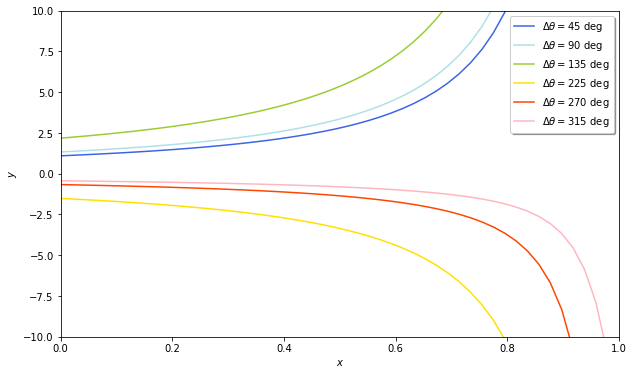
\includegraphics[width=\linewidth]{static/tof_curves/tof_gauss.png}
  \caption{Gauss 1809 time of flight curves for various transfer angles. This
  figure was obtained for $\rho=r_2/r_1=2$ with unitary $\mu$ and $\Delta t$.}
    \label{fig:tof_gauss}
\end{figure}

For solving the value of $x$, an initial guess about $y$ needs to be made, such
that $y_0=1.00$ for example. Then, the value of $x(y_0)$ is solved via equation
\ref{eq:gauss_equations} so a new value of $X(x)$ can be computed. Finally, a new
value of $y(x)$ is found. This value is compared with the initial one $y_0$ used
for the iteration. If $\norm{y - y_0} < \text{atol}$, then the method has
converged and the value for the free-parameter has been found. In figure
\ref{fig:tof_gauss}, the relation between the $x$ and $y$ parameter is shown
graphically for various transfer angles. The singular ones, such us any multiple
of $2\pi$ and $\pi$ have been omitted.

Finally, \cite{bate1971} suggests to use the semi-latus rectum for computing the
$f$ and $g$ functions, so the velocity vectors at the initial and final
positions can be obtained.

The decision to include this solver within the performance comparison was based
on two facts: the main one is its classic nature, so the solutions provided by
modern solvers can be better seen, the later is that \cite{sec:battin_solver}
improved this solver.


\subsection{Battin 1984}
\label{sec:batin_solver}

Batin is one of the author's who has devoted a lot of time reviewing and
studying the Lambert's problem. Chapters 6 and 7 from his book \citetitle{battin1999}
cover the whole geometry of the problem while provide a new algorithm following
the approach initiated by Gauss. Even if appearing in the book, this algorithm
is the result of a PhD thesis developed by Vaughan, under the supervision of
Battin, see \cite{vaughan1983}. The algorithm was published by both just a year
later in \cite{battin1984} and it is usually known as the Battin-Vaughan solver.

This new algorithm moves the singularity for transfer angles of $180$ degrees to
the less usual case of $360$ degrees. Although it no longer makes use of ratio
of sector to triangle areas, the notation used in the equations and the solution
procedures is quite similar to the solver devised by Gauss. No only that, this
solver is capable of fully working with all possible geometries and it is known
to have a better accuracy and robustness than Gauss one.

The so-called Battin's first and second equation, again following the ideas
introduced by Gauss, are given by expressions in \ref{eq:battin_equations}:

\begin{equation}
  x = \sqrt{\left(\frac{1 - l}{2} \right)^{2} + \frac{m}{y^2}} - \frac{1+l}{y^2}\quad\quad\quad
  y^3 - y^2 - h_1(x)y^2 - h_2(x) = 0
  \label{eq:battin_equations}
\end{equation}

where the auxiliary variables are given by \ref{eq:aux_battin}:

\begin{equation}
	\lambda = \pm \frac{\sqrt{s(s-c)})}{s}\quad\quad
	l = \left(\frac{1 - \lambda}{1 + \lambda}\right)^2\quad\quad\quad
	m = \frac{8\mu \Delta t^2}{s^3(1 + \lambda)^6}
	\label{eq:aux_battin}
\end{equation}

and the $h$ functions can be evaluated using expression \ref{eq:h_coeff}:

\begin{equation}
	h_1 = \frac{(l+x)^2(1 + 3x + \xi)}{(1+2x+l)(4x + \xi(3+x))}\quad
	h_2 = \frac{m(x-l+\xi)}{(1+2x+l)(4x + \xi(3+x))}
	\label{eq:h_coeff}
\end{equation}

being $\xi$ computed from a continued fraction defined in the original Battin's
article but simplified to:

\begin{equation}
  \xi(x) =
  \begin{cases}
	  \frac{4x(1 - \text{ATANR}(x))}{(3 +x)\text{ATANR}(x) - 3} &
	  \text{$x\neq0$}\\
	  5 & \text{$x = 0$}
  \end{cases}
\end{equation}

where the function $\text{ATANR}$ is an hypergeometric function defined as:

\begin{equation}
  \text{ATANR} = F(\frac{1}{2}, 1, \frac{3}{2}, -x) =
  \begin{cases}
	  \frac{\arctanh{\sqrt{-x}}}{\sqrt{-x}} & \text{$-1 < x < 0$}\\
	  1 & \text{$x = 0$} \\
	  \frac{\arctan{\sqrt{x}}}{\sqrt{x}} & \text{$x > 0$}
  \end{cases}
\end{equation}

following \cite{allen2015} article. This approach is cited here as
implementing continued fractions in a computer might be a bit tricky, leading to
non-optimized code. Modern computers do not struggle with the computations of
trigonometric functions as in the old days.

\vspace{0.5cm}
\begin{figure}[h]
  \centering
  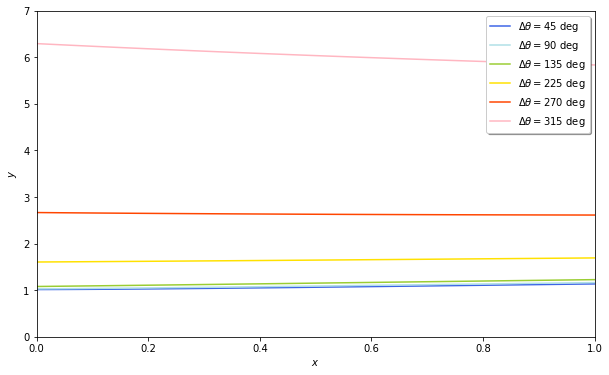
\includegraphics[width=\linewidth]{static/tof_curves/tof_battin.png}
  \caption{Battin 1984 time of flight curves for various transfer angles. This
  figure was obtained for $\rho=r_2/r_1=2$ with unitary $\mu$ and $\Delta t$.}
  \label{fig:tof_battin}
\end{figure}


Battin also improved previous equations at the end of his report to improve even
more the convergence of the method, so reader is encouraged to review them. The
implementation of the solver corresponds to these cited approach. The procedure
when solving the free-parameter $x$ is the same one as for the Gauss solver.
Curves for the time of flight are given figure \ref{fig:tof_battin}.

This solver was selected considering its enhancements over the Gauss one. Not
only that, it is one of the most moderns of the semi-latus rectum based solvers,
see subsection \ref{sec:p_solvers}.


\subsection{Gooding 1990}

The algorithm by \cite{gooding1990} was considered to have a high performance,
as claimed in performance reports of its days such us \cite{klumpp1999}. This is
the main reason behind its selection for the performance comparison.

Gooding's solver is based on the universal formulation branch, presented in
\ref{sec:universal_solvers}. This formulation enables to solve for elliptic,
parabolic or hyperbolic orbits without splitting the workflow into an excessive
amount of sections. Gooding's inherit from \cite{lancaster1970} solver and
dramatically improves its convergence and accuracy up to thirteen decimal
places.

The equation relating the canonical time of flight, named $T$ in Gooding's
article, and the free-parameter $x$ is complex. The equations collected by
\cite{torre2015} have been very useful and presented in \ref{eq:gooding_T}:

\begin{equation}
  \Delta t = 
  \begin{cases}
    4/3(1 - q^3) & \text{Parabolic solution}\\
    \sigma_x(f(x)) - q^3\sigma_x(q^2f(x)) & \text{Near-parabolic}\\
    \frac{2}{E(x)}\left(x - \lambda z(x) - \frac{d(x)}{y(x)}\right) & \text{Lancaster and Blanchard}
  \end{cases}
  \label{eq:gooding_T}
\end{equation}

Gooding's solver makes use of a bi-linear initial guess, which makes the initial
iteration value for the free-parameter to be closer to the final solution.
Together with the usage of a Halley's method, the convergence of the method is
quite fast. The construction of the velocity vectors is made using the radial
and tangential components. The curves for the time of flight, in figure
\ref{fig:tof_gooding}, are exactly the same ones as \cite{lancaster1970}, since
Gooding only devised and improved algorithm and did not introduce any additional
steps.

\vspace{0.5cm}
\begin{figure}[h]
  \centering
  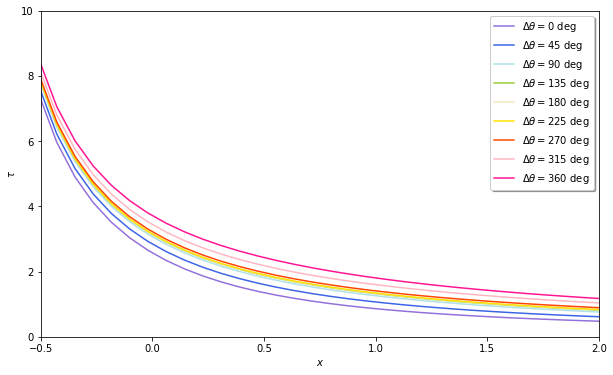
\includegraphics[width=\linewidth]{static/tof_curves/tof_gooding.png}
  \caption{Gooding 1990 time of flight curves for various transfer angles. This
  figure was obtained for $\rho=r_2/r_1=2$ with unitary $\mu$ and $\Delta t$.
  Only the direct transfer region is shown for the purposes of this work.}
  \label{fig:tof_gooding}
\end{figure}


\subsection{Avanzini 2008}

Among the different Lambert's problem solvers, the one devised by
\cite{avanzini2008} truly unleashes the geometry of the problem. This solver is
the very first of its branch within the set of eccentricity based ones, see
subsection \ref{sec:ecc_solvers}. By exploiting the conservation of the
eccentricity vector projection onto the chord one, it is able to solve for the
problem no matter the geometry of the orbit.

Avanzini's starts defining the fundamental eccentricity of the orbit $e_F$ (the
component along the chord direction) and the transverse one $e_T$. This is the
one which will be used as free-parameter. The relations given by
\ref{eq:ecc_avanzini} apply:

\begin{equation}
	e_F = \frac{\norm{\vec{r_1}} - \norm{\vec{r_2}}}{\norm{\vec{c}}}\quad\quad
	\norm{\vec{e}} = \sqrt{e_F^2 + e_T^2}
	\label{eq:ecc_avanzini}
\end{equation}

The free-parameter is defined as:

\begin{equation}
  x =
  \begin{cases}
    \frac{e_P e_H}{e_P + e_H}\log{\left(\frac{e_P(e_T + e_H)}{e_H(e_P - e_T)}\right)} & \text{if $\Delta \theta < \pi$}\\
    -e_P \log{\left(1 - \frac{e_T}{e_P} \right)} & \text{if $\Delta \theta > \pi$}
  \end{cases}
\end{equation}

where $e_P$, and $e_H$ can be computed using expressions \ref{eq:ecc_aux}:

\begin{equation}
  e_P = \sqrt{1 - e_F^2}\quad\quad\quad
  e_H = \sqrt{(e_\text{max}^2 - e_F^2)}\quad\quad
  e_\text{max} = \frac{-1}{\cos{\Delta \theta / 2}}
  \label{eq:ecc_aux}
\end{equation}

with all previous relations, it is possible to estimate the value of the
transverse eccentricity from the free-paramter $x$ by making use of equation
\ref{eq:ecc_T_avanzini}

\begin{equation}
  e_T =
  \begin{cases}
    e_P e_H \frac{X - 1}{e_p + e_H X} \text{if $\Delta \theta < \pi$}\\
    e_P \left(1 - \exp{\left(\frac{-x}{e_P} \right)} \right)
  \end{cases}
  \label{eq:ecc_T_avanzini}
\end{equation}

being $X$ defined as:

\begin{equation}
	X = \exp{\left(\left(\frac{1}{e_H} + \frac{1}{e_P} \right)x\right)}
\end{equation}

The starting value to be used for $x$ was imposed by Avanzini to be $x_0 = 0$.
The root solver declared by this author was the secant method, see subsection
\ref{sec:numerical_method}.

\vspace{0.5cm}
\begin{figure}[h]
  \centering
  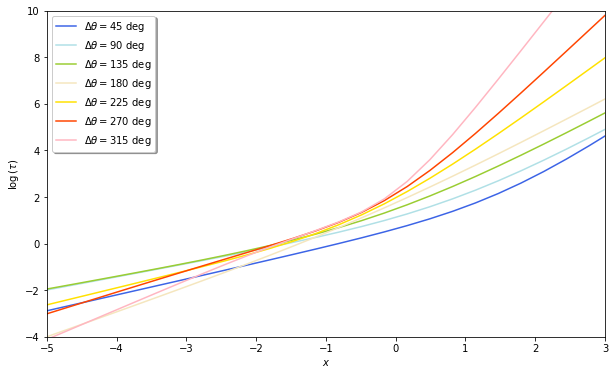
\includegraphics[width=\linewidth]{static/tof_curves/tof_avanzini.png}
  \caption{Avanzini 2008 time of flight curves for various transfer angles. This
  figure was obtained for $\rho=r_2/r_1=2$ with unitary $\mu$ and $\Delta t$.}
  \label{fig:tof_avanzini}
\end{figure}

Once the value of $x_0$ is known, the one for $e_T$ can be computed and then
the eccentricity of the orbit $e$, as the fundamental component is already
known. Therefore, to check if the value of $x_0$ is the right one, the current
time of flight and the one coming from the evaluation of Kepler's equation are
compared within some tolerance. As happens with other solvers, if the distance
between the two values is excessive, a correction is made to the free-parameter
and a new iteration begins till the method converges.

This solver was included due to its simplicity together with the fact of being
the first one of its class.

\subsection{Arora 2013}

Some years ago, \cite{arora2013} published a new Lambert's solvers based on a
cosine transformation. The new algorithm was strongly influenced by
\cite{bate1971} one and compared in performance against \cite{gooding1990} one
in Arora's publication. This solver belongs to the \ref{sec:universal_solvers}
set.

Arora introduced the $k$ free-paramter, which is related to the eccentric and
hyperbolic anomalies. The canonical time of flight can be computed as:

\begin{equation}
	\text{TOF} = S\sqrt{1 - k\tau}(\tau + (1 - k\tau)W)
\end{equation}

where the auxiliary parameters $\tau$, $S$ and $W$ are obtained via:

\begin{equation}
  S = \sqrt{\frac{(\norm{\vec{r_1}} + \norm{\vec{r_2}})^3}{\mu}}\quad\quad
  W = \frac{q}{\sqrt{m ^3}} - \frac{k}{m}\quad\quad
  m = 2 - k^2
\end{equation}

Avanzini improved the convergence of the method by converting some expressions
into series expansion- However, the core of this solver lies in the strong and
robust initial guess procedure devised by the author. Although based on a
rational-formulae (arbitrary initial guess), the solver rapidly converges in a
couple of iterations to the final solution.

The solution procedure is similar to Avanzini's solver, in the sense that
Kepler's equation is evaluated for various values of $k$ till it matches the
current time of flight.

The algorithm was also devised for working within the multi-revolution scenario
but as introduced early, the analysis of this region is out of the scope of this
work. Therefore, the curves for the time of flight for this solver presented in
figure \ref{fig:tof_arora} only show the direct transfer region.

\vspace{0.5cm}
\begin{figure}[h]
  \centering
  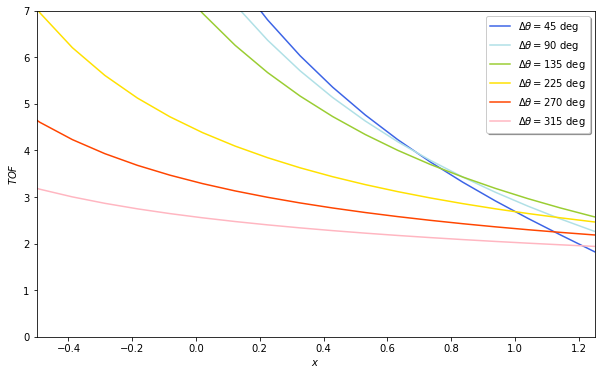
\includegraphics[width=\linewidth]{static/tof_curves/tof_arora.png}
  \caption{Arora 2013 time of flight curves for various transfer angles. This
  figure was obtained for $\rho=r_2/r_1=2$ with unitary $\mu$ and $\Delta t$.}
  \label{fig:tof_arora}
\end{figure}

The numerical method used by Arora is Halley's one and the subroutine for the
computation of the initial and final velocity vectors is made using the $f$ and
$g$ functions.


\subsection{Vallado 2013}

One of the most popular books about modern astrodynamics is the
\citetitle{vallado2013} by which also provides different pseudo-code for
implementing a variety of useful computer algorithms related with orbital
mechanics. One of these algorithms was an improved version of the
\cite{bate1971} universal one, for which Vallado imposed a bisection method. By
doing so, the method is ensured to converge no matter the type of orbit.

Vallado introduces the $\psi$ variable as the free-parameter. This variable is
related to the universal Kepler's equation via equation \ref{eq:tof_vallado}:

\begin{equation}
  t = \frac{\chi^3 c_3 + A \sqrt{y}}{\sqrt{\mu}}
  \label{eq:tof_vallado}
\end{equation}

where the variables $\chi$ and $y$ are given by:

\begin{equation}
  \chi = \sqrt{\frac{y}{c_2}}\quad\quad
  y = \norm{\vec{r_1}} + \norm{\vec{r_2}} + \frac{A(\psi + c_3 - 1)}{\sqrt{c_2}}
\end{equation}

and the transfer angle parameter $A$ is computed as:

\begin{equation}
  A = 
  \begin{cases}
    \sqrt{\norm{\vec{r_1}} \norm{\vec{r_2}} (1 + \cos{(\Delta \theta)})} & \text{if $\Delta \theta < \pi$}\\
    -\sqrt{\norm{\vec{r_1}} \norm{\vec{r_2}} (1 + \cos{(\Delta \theta)})} & \text{if $\Delta \theta > \pi$}\\
  \end{cases}
\end{equation}

In previous equations, the values for the $c_2$ and $c_3$ variables can be
computed using the corresponding Stumpff coefficients evaluated at a particular
value of $\psi$.

\vspace{0.5cm}
\begin{figure}[h]
  \centering
  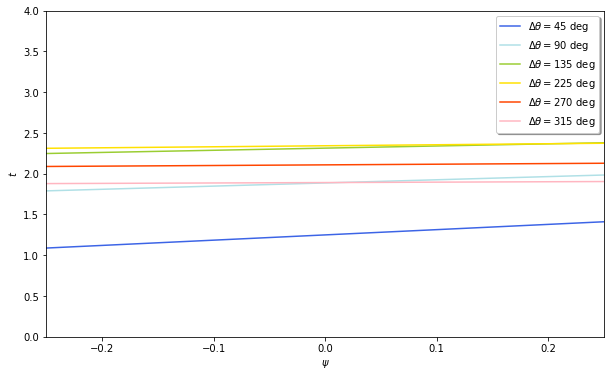
\includegraphics[width=\linewidth]{static/tof_curves/tof_vallado.png}
  \caption{Vallado 2013 time of flight curves for various transfer angles. This
  figure was obtained for $\rho=r_2/r_1=2$ with unitary $\mu$ and $\Delta t$.}
  \label{fig:tof_vallado}
\end{figure}

Similarly to other solvers, the goal is to iterate on the free-parameter till
the time computed using the universal Kepler's equation is equal to the expected
one imposed by the statement of the problem within some tolerance. Because this
method makes use of bisection, the solution is guaranteed to converge always.
However, a huge number of iterations is required for the solver to achieve
accurate results.

This method is belongs to the same branch as the one for \cite{arora2013}, see
the diagram from subsection \ref{sec:universal_solvers}. Therefore, Vallado's
solver was selected due to its simplicity against Arora's one so a performance
can be between them. 

\subsection{Izzo 2015}

The last of the solvers for this work is the one devised by \cite{izzo2015}.
This solver quickly became popular because it enhanced \cite{lancaster1970} and
\cite{gooding1990} ones by introducing one last change of variable. Not only
that, the Halley's method was upgraded to a Householder's one while the initial
guess made use of a linear approximation instead of a bi-linear one.

Izzo's solver belongs to the \ref{sec:universal_solvers} and names the
free-parameter $\xi$. This variable is related to Gooding's one $x$ via the
transformation given in \ref{eq:izzo_gooding}:

\begin{equation}
  \xi = 
  \begin{cases}
    \log{(1 + x)} & \text{if $M=0$}\\
    \log{\left(\frac{1+x}{1-x} \right)} & \text{if $M>0$}
  \end{cases}
  \label{eq:izzo_gooding}
\end{equation}

Regarding the non-dimensional time of flight, this variable is also modified
making use of expression \ref{eq:izzo_tof}:

\begin{equation}
  \tau = \log{(T)}
  \label{eq:izzo_tof}
\end{equation}

Izzo had to deal with the computation of the high-order derivatives of $\tau$
with respect to $\xi$. These are not provided here but can be checked in the
original report.

All previous modifications, ended up showing the relation between the
free-parameter and non-dimensional transfer angle which is presented in figure
\ref{fig:tof_izzo}.

\vspace{0.5cm}
\begin{figure}[h]
  \centering
  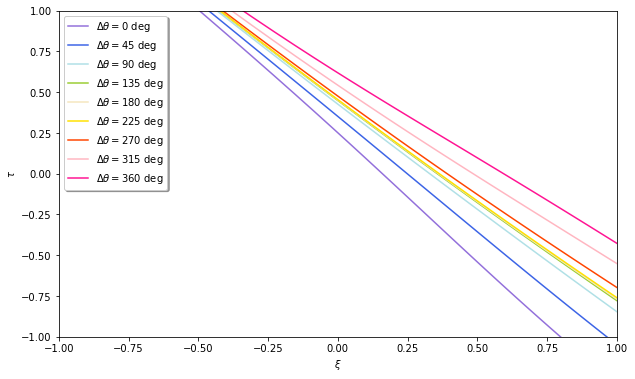
\includegraphics[width=\linewidth]{static/tof_curves/tof_izzo.png}
  \caption{Izzo 2015 time of flight curves for various transfer angles. This
  figure was obtained for $\rho=r_2/r_1=2$ with unitary $\mu$ and $\Delta t$.}
  \label{fig:tof_izzo}
\end{figure}

\section{Comparative table of elements}

After introducing all solvers in a more detailed way, it is convenient to
collect all the information an present it to reader in a more compact way. This
is the goal of table \ref{table:elements} provided at the end of this section, in which the different
elements and steps used by each solver have been collected.

Although the free-parameters are various, it is possible to see some common
elements between the selected modern solvers. For example, those ones using a
numerical method make use of high order one to ensure quick convergence or a
bounded one, so the solution is always achieved. Not only that, for the velocity
vectors construction, the preferred approach seems to be through the usage of
$f$ and $g$ functions. Regarding the initial guess, rational formulae is the
most popular among the solvers presented in this work. Other initial guess
procedures like linear or bi-linear can also be found.

\begin{table}[H]
  \footnotesize
  \centering
  \begin{tabular}{|c|c|c|c|c|}
    \hline
    \multirow{2}{*}{\textbf{Method}} & \multicolumn{4}{c|}{\textbf{Step}}                                                                                             \\ \cline{2-5}
                                     & \textbf{Free-parameter}            & \textbf{Initial guess} & \textbf{Numerical method} & \textbf{$\vec{v_1}$ and $\vec{v_2}$} \\ \hline
    Gauss 1809                       & $x$                                & Rational formulae      & System of equations       & $f$ and $g$                          \\ \hline
    Battin 1984                      & $x$                                & Rational formulae      & System of equations       & $f$ and $g$                          \\ \hline
    Gooding 1990                     & $x$                                & Bi-linear              & Halley's method           & $v_{r_i}$ and $v_{t_i}$              \\ \hline
    Avanzini 2008                    & $e_T$                              & Interval               & Regula-falsi              & COE to RV                            \\ \hline
    Arora 2013                       & $k$                                & Rational formulate     & Halley's method           & $f$ and $g$                          \\ \hline
    Vallado 2013                     & $\psi$                             & Interval               & Bisection                 & $f$ and $g$                          \\ \hline
    Izzo 2015                        & $\xi$                              & Linear                 & Householder's method      & $v_{r_i}$ and $v_{t_i}$              \\ \hline
  \end{tabular}
  \caption[Basic elements of each selected solver.]{Basic elements of each selected solver.}
  \label{table:elements}
\end{table}

\section{Performance comparison}

This section is the core of this work. In here, all the metrics developed and
used for the carrying out the performance comparison are explained in detail
together with the justification on why they were selected.

All the simulations were performed considering a non-dimensional radius of
$\rho=\norm{\vec{r_2}}/\norm{\vec{r_1}}=2$ and unitary gravitational parameter
$\mu=1$ [L3, T2], where L3 and T2 stand for units of cubic length and squared
time respectively. The problem was solved for a variety of transfer angles
$\Delta \theta$ between $0$ and $2\pi$ and non-dimensional transfer times $\tau$
within the same range of values. For this last parameter, equation
\ref{eq:non_dimensional_tof}:

\begin{equation}
  \tau =  \Delta t \cdot \sqrt{\frac{8\mu}{s^3}}
  \label{eq:non_dimensional_tof}
\end{equation}

By making use of previous equation, each revolution solution lies within an
interval which is a multiple of $2\pi$. For example, the direct transfer problem
will have the solution within the $[0, 2\pi)$ interval, while for the
multiple-revolution scenario, the interval changes to $[2\pi M, 2\pi(M+1))$.

As it has been introduced in several sections, this work only covers the direct
arc transfer, meaning that the multi-revolution scenario is not studied. All
orbits were assumed to be \textit{prograde} and no distinction between
\textit{low} or \textit{short} paths was required as multiple solutions only
appear in the multi-revolution problem. The absolute tolerance was set to $1e-5$
and the relative one to $1e-7$.

The three metrics used in this report are:

\begin{itemize}
  \item \textbf{Number of iterations}: this metric provides information about
        the convergence of the numerical method but also about the initial
        guess. Because the initial guess outputs an estimate solution, the
        accurate this routine is, the lower the amount of iterations required
        by the numerical method.
  \item \textbf{Time per iteration}: which measures the mean time required for
        computing a new approximate value of the free-parameter. This metric
        reveals more information about the time consumed by the numerical
        method.
  \item \textbf{Total computation time}: which computes the total time required
	by the algorithm when computing the solution to the problem. When
	comparing this value to the time employed for the iteration workload, it
	is possible to identify bottlenecks and weak implementation points.
\end{itemize}

\subsection{Number of iterations}

The first metric used for the performance comparison is the amount of iterations
it takes for a solver to achieve the solution for a given combination of $\Delta
  \theta$ and $\Delta \tau$. Black regions show for which points the algorithm did
not converged, either because of the accuracy or the method itself.

Gauss' solver, in figure \ref{fig:iter_gauss}, reveals that the method is only
valid for lower transfer angle and non-dimensional times. This situation was
already known and claimed by several authors in literature. On the other hand,
the improved version of the method by Battin, see \ref{fig:iter_battin}
converges for any case and the imposed absolute tolerance. These last method is
seen to be more robust and accurate than Gauss one.

The solver devised by Gooding shows an stable behavior for most of the solution
space, only requiring between two and three iterations, \ref{fig:iter_gooding}.
This is due to the strong initial guess together with the usage of Halley's
method.

Regarding Avanzini's solver, this algorithm exhibits a lower number of
iterations for transfer angles of the same value of the non-dimensional time of
flight. For corner cases, see \ref{fig:iter_avanzini}, the iterations increase up
to eight or nine. Even with that, the solution is found in all of the cases,
meaning that the algorithm converged without any problem.

Arora's algorithm, in figure \ref{fig:iter_arora}, is seen to be the most stable
one, requiring a mean of only two iterations. This algorithm holds the most
complex initial guess procedure of all the solvers presented in this work, which
together with Halley's method explains the lower amount of iterations.
Convergence is ensured with this solver.

Vallado's solver also converged to the majority of the cases, except for those
ones with low time of flight. However, due to the bisection method employed, the
number of iterations increases dramatically. This can be seen in figure
\ref{fig:iter_vallado}.

Finally, Izzo's solver in figure \ref{fig:iter_izzo} is also seen to be stable
and robust for the majority of the cases. Only values around $\tau=\pi/2$
require more than two iterations, no matter the transfer angle.


% --- START: NUMBER OF ITERATIONS FIGURES ---
\begin{figure}[H]
  \begin{minipage}{0.48\textwidth}
    \centering
    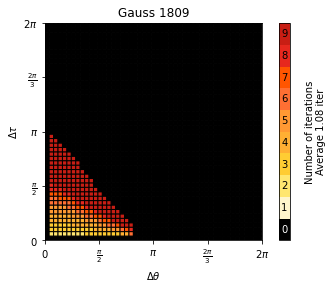
\includegraphics[width=1.05\linewidth]{static/iter/iter_gauss_1809.png}
    \caption{Gauss' iterations.}\label{fig:iter_gauss}
  \end{minipage}\hfill
  \begin{minipage}{0.48\textwidth}
    \centering
    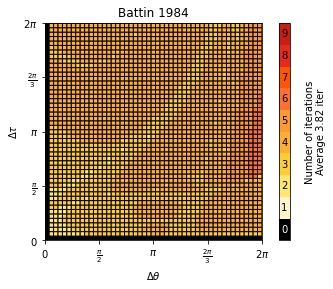
\includegraphics[width=1.05\linewidth]{static/iter/iter_battin_1984.png}
    \caption{Battin's iterations.}\label{fig:iter_battin}
  \end{minipage}
\end{figure}

\begin{figure}[H]
  \begin{minipage}{0.48\textwidth}
    \centering
    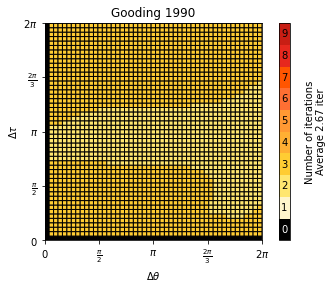
\includegraphics[width=1.05\linewidth]{static/iter/iter_gooding_1990.png}
    \caption{Gooding' iterations.}\label{fig:iter_gooding}
  \end{minipage}\hfill
  \begin{minipage}{0.48\textwidth}
    \centering
    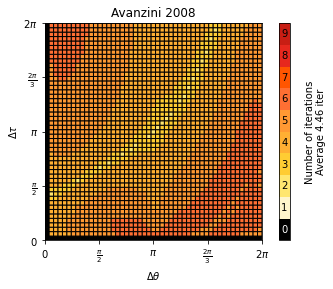
\includegraphics[width=1.05\linewidth]{static/iter/iter_avanzini_2008.png}
    \caption{Avanzini's iterations.}\label{fig:iter_avanzini}
  \end{minipage}
\end{figure}

\begin{figure}[H]
  \begin{minipage}{0.48\textwidth}
    \centering
    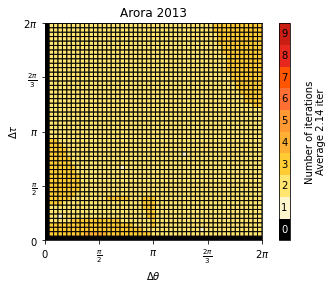
\includegraphics[width=1.05\linewidth]{static/iter/iter_arora_2013.png}
    \caption{Arora' iterations.}\label{fig:iter_arora}
  \end{minipage}\hfill
  \begin{minipage}{0.48\textwidth}
    \centering
    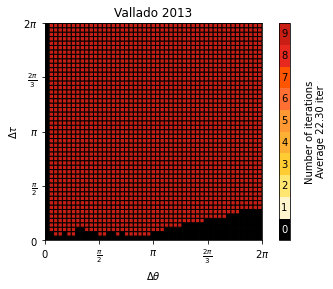
\includegraphics[width=1.05\linewidth]{static/iter/iter_vallado_2013.png}
    \caption{Vallado's iterations.}\label{fig:iter_vallado}
  \end{minipage}
\end{figure}

\begin{figure}[H]
  \begin{minipage}{0.48\textwidth}
    \centering
    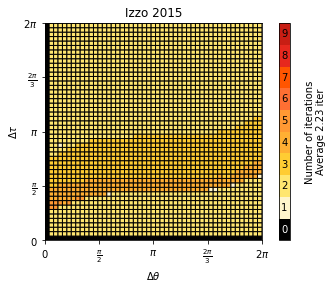
\includegraphics[width=1.05\linewidth]{static/iter/iter_izzo_2015.png}
    \caption{Izzo's iterations.}\label{fig:iter_izzo}
  \end{minipage}\hfill
  \begin{minipage}{0.48\textwidth}
    \centering
    
\includegraphics[width=1.05\linewidth]{static/void_figure.png}
  \end{minipage}
\end{figure}
% --- END: NUMBER OF ITERATIONS FIGURES ---

\subsection{Time per iteration}

A solver may require a huge number of may require a huge number of iterations.
However, if each one of those only needs a minimum amount of time, the overall
computation might be a high performance one. In this subsection, the time per
iteration of each one of the solvers is presented.

It is important to state that the time required for a computer to solve a
particular problem might slightly vary due to internal processes which have
nothing to do with the computation process itself. Therefore, the problem was
solved multiple times and the mean iteration time. Let us now present the
results.

For the case of Gauss' solver, the time consumed per iteration is stable as
depicted by figure \ref{fig:tpi_gauss}. On the other hand, Battin's solver in
figure \ref{fig:tpi_battin} shows a reduction in the time per iteration for low
values of the canonical transfer time. However, this last solver requires more
time than Gauss one due to the complexity of the method used. Nevertheless, it
converges for all cases, which is a major advantage over speed as a solution is
found.

Gooding's solver in \ref{fig:tpi_gooding} only shows an critical region near
non-dimensional times of $\tau=\pi/2$. For the rest of the cases, the time per
iteration is quite low and stable. Halley's method is proof to be fast when
carrying out the iteration workload.

The algorithm requiring the greatest amount of time per iteration is Avanzini's
one, see figure \ref{fig:tpi_avanzini}. This solver requires more time for the
regions in which it employed less iterations.

Arora's solver, on the other hand, shows an overall time per iteration slightly
greater than Gooding's one. Even with that, the solver only experiences an
increase in the computation of the time per iteration for values below of
$\tau=\pi/2$. The diagram for this solver is shown in figure
\ref{fig:tpi_arora}.

Vallado's solver, in figure \ref{fig:tpi_vallado} shows now a closer behavior
to the rest of the solvers when discussing the time per iteration. This is due
to the bisection method employed by the solver, as this root solver is fast from
the time per iteration point of view but requires a huge amount of iterations
for achieving the desired absolute tolerance.

The last of the solvers, Izzo's one in figure \ref{fig:tpi_izzo} is not as
stable as Gooding's or Arora's algorithms, but also shows a great stability and
performance for the iteration workload. As similar to Arora's, this solver
experiences and increase in the time per iteration for values of $\tau=\pi/2$.


% --- START: NUMBER OF TIME PER ITERATION FIGURES ---
\begin{figure}[H]
  \begin{minipage}{0.48\textwidth}
    \centering
    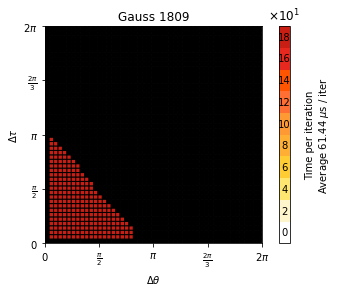
\includegraphics[width=1.05\linewidth]{static/tpi/tpi_gauss_1809.png}
    \caption{Gauss' time per iteration.}\label{fig:tpi_gauss}
  \end{minipage}\hfill
  \begin{minipage}{0.48\textwidth}
    \centering
    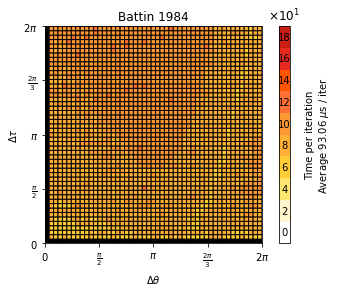
\includegraphics[width=1.05\linewidth]{static/tpi/tpi_battin_1984.png}
    \caption{Battin's time per iteration.}\label{fig:tpi_battin}
  \end{minipage}
\end{figure}

\begin{figure}[H]
  \begin{minipage}{0.48\textwidth}
    \centering
    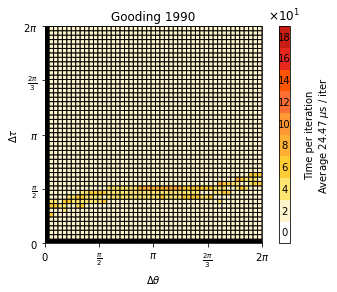
\includegraphics[width=1.05\linewidth]{static/tpi/tpi_gooding_1990.png}
    \caption{Gooding' time per iteration.}\label{fig:tpi_gooding}
  \end{minipage}\hfill
  \begin{minipage}{0.48\textwidth}
    \centering
    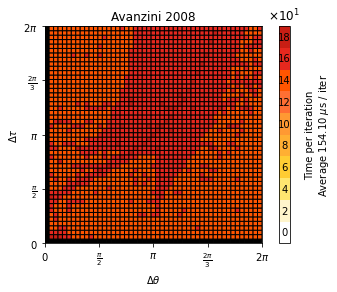
\includegraphics[width=1.05\linewidth]{static/tpi/tpi_avanzini_2008.png}
    \caption{Avanzini's time per iteration.}\label{fig:tpi_avanzini}
  \end{minipage}
\end{figure}

\begin{figure}[H]
  \begin{minipage}{0.48\textwidth}
    \centering
    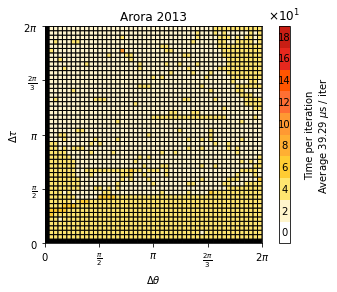
\includegraphics[width=1.05\linewidth]{static/tpi/tpi_arora_2013.png}
    \caption{Arora' time per iteration.}\label{fig:tpi_arora}
  \end{minipage}\hfill
  \begin{minipage}{0.48\textwidth}
    \centering
    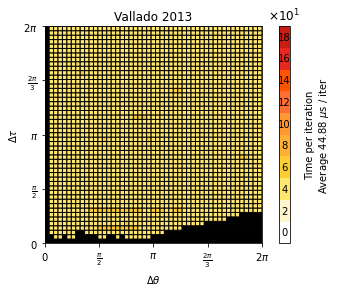
\includegraphics[width=1.05\linewidth]{static/tpi/tpi_vallado_2013.png}
    \caption{Vallado's time per iteration.}\label{fig:tpi_vallado}
  \end{minipage}
\end{figure}

\begin{figure}[H]
  \begin{minipage}{0.48\textwidth}
    \centering
    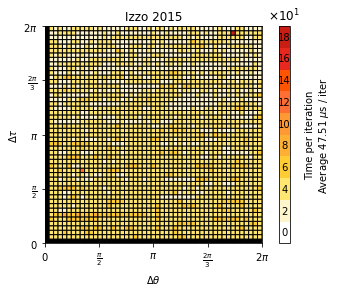
\includegraphics[width=1.05\linewidth]{static/tpi/tpi_izzo_2015.png}
    \caption{Izzo's time per iteration.}\label{fig:tpi_izzo}
  \end{minipage}\hfill
  \begin{minipage}{0.48\textwidth}
    \centering
    
\includegraphics[width=1.05\linewidth]{static/void_figure.png}
  \end{minipage}
\end{figure}
% --- END: TIME PER ITERATION FIGURES ---


\subsection{Total computation time}

Finally, the total computation time employed by the algorithm for computing the
whole problem is presented. Because the amount of iterations required and the
time per iterations are known, it is possible to compute the percentage of the
time spent during the iteration workload. The idea is that the main workload of
a solver should be located within the iteration process itself and not in the
initial guess computation, the construction of the velocity vectors or function
calls. Again, it must be pointed out that background processes running on local
machine can affect the computation time. 

Gauss' solver exhibits a high total computation time, see figure
\ref{fig:ttc_gauss} even if its time per iteration is low. This means that the
algorithm requires lots of iterations to reach an accurate solution. The
improved version devised by Battin performs much better, as depicted in figure
\ref{fig:ttc_battin}. However, these two algorithms are far from being fast when
computing the solution.

Gooding's solver performs much better in total time than Gauss or Battin
algorithms. The figure in \ref{fig:ttc_gooding} is proportional to previous
results for the number of iterations and time per each one of those. In
addition, a bottlenecks is identified for transfer times near $\tau=\pi/2$.

On the other hand, Avanzini's solver has a huge time cost as seen in figure
\ref{fig:ttc_avanzini}. When comparing this result with previous figures in
\ref{fig:iter_avanzini} and \ref{fig:tpi_avanzini}, an implementation issue
might be the reason behind this. Because the Kepler's equation becomes complex
when written as function of the transverse eccentricity, a simplification making
use of function calls was made. The excessive calls to these function are
probably the reason behind this total computation time results. The usage of a
high-order method might be also a good strategy for reducing the computation time.

Arora's solver presents a very low computation time when compared to the rest of
the solvers. Not only that, a uniform value is found for every combination of
the transfer angle and the canonical time of flight, being not possible to
identify any bottlenecks on figure \ref{fig:ttc_arora}.

Vallado's algorithm, due to bisection method again, is seen to be detrimental
for this algorithm, see the results in figure \ref{fig:ttc_vallado}. However, as
pointed by its author, it converges to the majority of the cases. A possible way
to improve this algorithm would be the introduction of a better initial guess or
mixed numerical solver.

Finally, Izzo's algorithm is the one requiring the lowest amount of time to
converge to the solution. The corner case for this solver was previously
identified during the number of iterations but no effect is seen in figure
\ref{fig:ttc_izzo}.

% --- START: NUMBER OF TOTAL TIME COMPUTATION FIGURES ---
\begin{figure}[H]
  \begin{minipage}{0.48\textwidth}
    \centering
    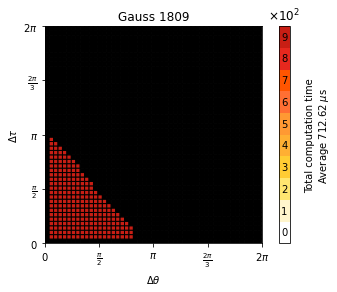
\includegraphics[width=1.05\linewidth]{static/ttc/ttc_gauss_1809.png}
    \caption{Gauss' total computation time.}\label{fig:ttc_gauss}
  \end{minipage}\hfill
  \begin{minipage}{0.48\textwidth}
    \centering
    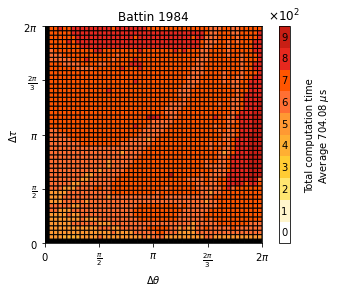
\includegraphics[width=1.05\linewidth]{static/ttc/ttc_battin_1984.png}
    \caption{Battin's total computation time.}\label{fig:ttc_battin}
  \end{minipage}
\end{figure}

\begin{figure}[H]
  \begin{minipage}{0.48\textwidth}
    \centering
    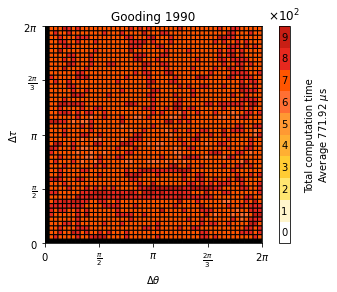
\includegraphics[width=1.05\linewidth]{static/ttc/ttc_gooding_1990.png}
    \caption{Gooding' total computation time.}\label{fig:ttc_gooding}
  \end{minipage}\hfill
  \begin{minipage}{0.48\textwidth}
    \centering
    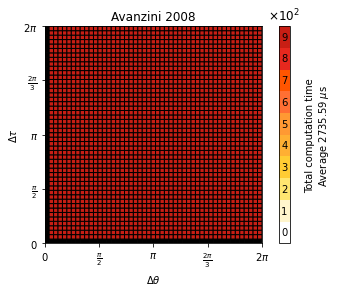
\includegraphics[width=1.05\linewidth]{static/ttc/ttc_avanzini_2008.png}
    \caption{Avanzini's total computation time.}\label{fig:ttc_avanzini}
  \end{minipage}
\end{figure}

\begin{figure}[H]
  \begin{minipage}{0.48\textwidth}
    \centering
    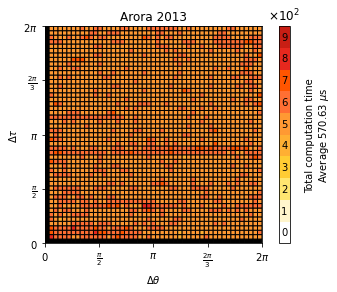
\includegraphics[width=1.05\linewidth]{static/ttc/ttc_arora_2013.png}
    \caption{Arora' total computation time.}\label{fig:ttc_arora}
  \end{minipage}\hfill
  \begin{minipage}{0.48\textwidth}
    \centering
    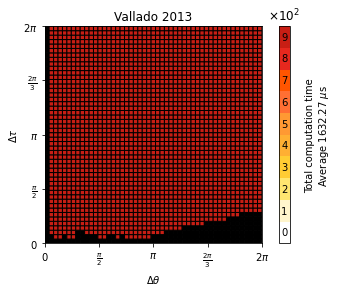
\includegraphics[width=1.05\linewidth]{static/ttc/ttc_vallado_2013.png}
    \caption{Vallado's total computation time.}\label{fig:ttc_vallado}
  \end{minipage}
\end{figure}

\begin{figure}[H]
  \begin{minipage}{0.48\textwidth}
    \centering
    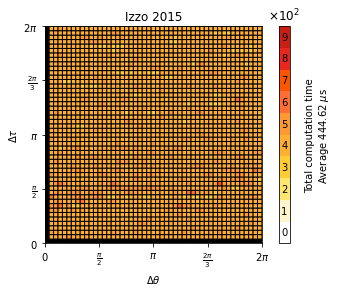
\includegraphics[width=1.05\linewidth]{static/ttc/ttc_izzo_2015.png}
    \caption{Izzo's total computation time.}\label{fig:ttc_izzo}
  \end{minipage}\hfill
  \begin{minipage}{0.48\textwidth}
    \centering
    
\includegraphics[width=1.05\linewidth]{static/void_figure.png}
  \end{minipage}
\end{figure}
% --- END: TOTAL TIME COMPUTATION ITERATION FIGURES ---



% ----------- END OF CONTENT FILES -------------


% Cite the bibliography
\printbibliography

\end{document}
